\documentclass[11pt]{article}
% We can write notes using the percent symbol!
% The first line above is to announce we are beginning a document, an article in this case, and we want the default font size to be 12pt
% \usepackage[utf8]{inputenc}
\usepackage[left=1.2in,top=.8in,right=1.2in,nohead,bottom=.5in]{geometry}
% This is a package to accept utf8 input.  I normally do not use it in my documents, but it was here by default in Overleaf.


\usepackage{amssymb,amsthm,amsmath}
\usepackage{commath,hyperref}
\usepackage{enumerate,xcolor}
\usepackage{natbib}
\usepackage{graphicx}
\usepackage{caption,setspace}
\usepackage{subcaption}
\DeclareMathOperator{\Tr}{Tr}
\newcommand{\dd}[1]{\mathrm{d}#1}
\newcommand{\E}{\mathbb{E}}
\newcommand{\Var}{\text{Var}}
\newcommand{\Cov}{\text{Cov}}
\newcommand{\X}{\mathcal{X}}
\newcommand{\B}{\mathcal{B}}
\newcommand\numberthis{\addtocounter{equation}{1}\tag{\theequation}}
% These three packages are from the American Mathematical Society and includes all of the important symbols and operations 
\usepackage{fullpage}
\usepackage{comment}
\usepackage[linesnumbered, ruled]{algorithm2e}
% By default, an article has some vary large margins to fit the smaller page format.  This allows us to use more standard margins.
\allowdisplaybreaks
\newtheorem{theorem}{Theorem}
\newtheorem{lemma}{Lemma}
\newtheorem{corollary}{Corollary}

\theoremstyle{remark}
\newtheorem{example}{Example}
\newtheorem{ass}{Assumption}
\newtheorem{remark}{Remark}
\setlength{\parskip}{0em}
\setlength{\parindent}{0in}
\renewcommand{\arraystretch}{1.5}

% This gives us a full line break when we write a new paragraph
% \usepackage[mathscr]{euscript}
% \usepackage{tikz}
% \newcommand*\circled[1]{\tikz[baseline=(char.base)]{
%             \node[shape=circle,draw,inner sep=2pt] (char) {#1};}}
% \newcommand{\indep}{\perp \!\!\! \perp}


\title{Globally-centered autocovariances in MCMC}

\author{
  Medha Agarwal \\
  Department of Mathematics and Statistics\\
  IIT Kanpur\\
  \texttt{medhaaga@iitk.ac.in} \and
 Dootika Vats \\
  Department of Mathematics and Statistics\\
  IIT Kanpur\\
  \texttt{dootika@iitk.ac.in}
}


\begin{document}

\maketitle


\onehalfspacing
\begin{abstract}
Autocovariances are the fundamental quantity in many features of Markov chain Monte Carlo (MCMC) simulations with autcorrelation function (ACF) plots being often used as a visual tool to ascertain the performance of a Markov chain. Unfortunately, for slow mixing Markov chains, the empirical autocovariance can highly underestimate the truth. For multiple chain MCMC sampling,  we propose a globally-centered estimate of the autocovariance that pools information from all Markov chains. We show the impact of these improved estimators in three aspects: (1) acf plots, (2) estimates of the Monte Carlo asymptotic covariance matrix, and (3) estimates of the effective sample size. 
\end{abstract}


% {\color{blue} Main things to change
% \begin{itemize}
%   \item I don't want to call this ``Replicated autocovariance'' or ``Replicated spectral variance''. I think ``Globally-centered autocovariance'' is more appropriate and self-explanatory. So we will have to go over the whole document and change this.

%   \item The contents are a bit messy right now, and I am having trouble organizing my thoughts. 

% \end{itemize}

% A rough outline of the organization
% \begin{enumerate}
%   \item Introduction, with a sneak peak at new plots. Change this example to a univariate mixture of Gaussians.:

%     Here, we will just explain the problem with the old ACF and what happens by using the new ACF. We will show a plot to illustrate the impact. Then we will summarize the three places this will have an impact: (1) ACF plots (2) estimators of the asymptotic variance-covariance matrix (3) estimating effective sample size.

%   \item Globally-centered autocovariance
%     \begin{itemize}
%       \item Theoretical soundness
%     \end{itemize}

%   \item Variance of Monte Carlo averages

%     Describe MC averages and CLT here and not before
%     \begin{itemize}
%       \item Globally-centered Spectral variance estimators
%       \begin{itemize}
%         \item Theoretical results
%         \item Fast implementation
%       \end{itemize}
%     \end{itemize}

%   \item Effective sample size

%   \item Examples

%   \item Discussion
%     \begin{itemize}
%       \item All plots have been made using the package:(name). The package can be found on GitHub.
%       \item One thing to discuss is that the new autocovariances can be used in the initial sequence estimators as well.
%     \end{itemize}

%   \item Appendix
%     \begin{itemize}
%       \item Proofs
%       \item ACF plots for other examples.
%     \end{itemize}

% \end{enumerate}
% }
% \newpage

\section{Introduction} \label{sec:intro}

Markov chain Monte Carlo (MCMC) is a sampling method used to obtain correlated realizations from a stochastic process. Due to this serial correlation in observations, a large number of MCMC samples are required to estimate features of the target distribution as compared to the independent ones. Therefore, it becomes imperative for an MCMC practitioner to have an idea about underlying dependence structure in the Markov chains. Autocovariance function (ACF) characterizes this dependence for a stationary Markov chain. Suppose $\{X_t; t \in \mathbb{Z}\}$ is a stochastic process with mean $\mu$ and follows second-order stationarity i.e. (1) $\mathbb{E}[X_t] = \mu$ is constant for all $t$, (2) $\mathbb{E}[X_t^2]$ is constant for all $t$, and (3) $\mathbb{E}[X_t X_{t+k}]$ is a function of $k$ only $\forall k,t \in \mathbb{Z}$. Then, the autocovariance function at lag-$k$ is defined as
%
\[
    \Gamma(k) = \Cov(X_t, X_{t+k}) = \mathbb{E}[(X_t - \mu)(X_{t+k} - \mu)^T].
\]

A popular sample autocovariance function is the empirical estimator. On a finite sample $X = (X_1, X_2, ..., X_n)^T$, the autocovariance at lag-$k$ is estimated as
%
\begin{equation} \label{eq:empirical_acf}
    \hat{\Gamma}(k) = \dfrac{1}{n}\sum_{t=1}^{n-\abs{k}}(X_t - \bar{X})(X_{(t+\abs{k})} - \bar{X})^T
\end{equation}


where $\bar{X} = \sum_{t=1}^nX_t/n$. Calculation of exact ACF has been done for simple models like autoregressive (AR), moving average (MA) (\cite{quenouille1947notes}), and autoregressive-moving-average (ARMA) (\cite{box2015time}) models. However, for most of the complex sampling algorithms, we rely on sample estimators for ACF. Unfortunately, the estimator given in equation \ref{eq:empirical_acf} has been observed to have a some drawbacks. Firstly, it is not immune to outliers (see \cite{ma2000highly}) and secondly, it is usually non-informative in case of slowly mixing Markov chains for decently finite samples. We address the second issue in this paper by using multiple representative samples of the target distribution via parallel Markov chains. With convenient multi-core computation resources, it is possible to get multiple Markov chains for a target distribution. Our goal is to combine the information from all the Markov chains while calculating the autocovariances\\

 A commonly faced problem with the MCMC models is the slow mixing property. In case of multi modal target distributions, it has been observed that the Markov chains tend to get \textit{stuck} in a particular mode for a long time. As a consequence, the chain fails to explore the sample space. In such situations, single chain empirical ACF will underestimate the autocovariance giving misleading inferences.  We propose an autocovariance estimator called globally-centered autocovariance function (G-ACF) with a simple fix in centering which has been observed to show drastically better results in many cases. We will further study the impact of G-ACF in calculation of two important applications of ACF (1) asymptotic variance of Markov chain average and (2) effective sample size (ESS).\\
 

 MCMC ensures asymptotic convergence, however this is not practically very useful where the number of samples is finite. There are many criteria for terminating simulation like fixed-time rule, sequencial fixed-volume rule (see \cite{glynn1992asymptotic}), and using Gelman Rubin diagnostics (\cite{gelman1992inference}). The relative fixed-volume rule has been thoroughly discussed for MCMC by \cite{flegal2015relative} and \cite{gong2016practical}. We will use method of effective sample size (ESS) by \cite{vats2019multivariate} for terminating the simulations. The quality of estimation of $\Sigma$ is critical in estimating their ESS. We will successfully show that the G-SVE estimates the truth better and prevents the premature stopping of Markov chain.\\

In the next section we introduce the new sample autocovariance estimator and calculate its bias for finite samples. We observe that the bias term for G-ACF is similar to the bias of empirical ACF except for a few small order end-effect terms that vanish as $n \to \infty$. In section \ref{sec:variance_est}, we introduce the globally-centered SVE and give a proof of strong consistency, bias, and variance calculations. We will elaborate on the estimator for ESS using G-SVE in section \ref{sec:ess}. Section \ref{sec:examples} gives an experimental study on three different examples for the proposed estimators. All the important proofs are given in the Appendix. 

\begin{example}[Demonstrative example]

We demonstrate the striking difference in the ACF plots through mixture of Gaussian target density using a random-walk Metropolis-Hastings sampler. The target density has two well separated and non-equal modes. Two Markov chains are started close to each mode. It can be seen in Figure \ref{fig:gaussian-trace} that for the first $10^4$ samples, the chains do not communicate with the other mode. Whereas for a sample size of $10^5$, the chains have jumped modes and therefore, a single chain can give reliable information about the distribution. We wish to make two points here: firstly, for small sample size, we observe that ACF gives extremely misleading estimates of autocovariance whereas G-ACF is very close to reality (Figure \ref{subfig:gauss-acf-1e4}). Whereas, sharing the information about Monte Carlo average across chains leads to better estimation of autocovariances. Secondly, for a large sample size, the estimates from G-ACF as well as ACF are equivalent. Figure \ref{subfig:gauss-trace_1e5} depicts the scenario when convergence is achieved. This shows that G-ACF is at least as good as ACF; hence safe to use in any setting.

\begin{figure}[htbp]
    \begin{subfigure}{.5\textwidth}
   \centering
   \includegraphics[width=\linewidth]{plots/gaussian-Targettrace_n1e4.pdf}
   \caption{$n = 10^4$}
   \label{subfig:gauss-trace_1e4}
 \end{subfigure}
 \begin{subfigure}{0.5\textwidth}
   \centering
   \includegraphics[width=\linewidth]{plots/gaussian-Targettrace_n1e5.pdf} 
   \caption{$n = 10^5$}
   \label{subfig:gauss-trace_1e5}
 \end{subfigure}
    \caption{Target density and Density plot for two chains starting at different values for a Gaussian mixture model with mixture probability $= 0.7, \; \mu_1 = -5, \; \mu_2 = 5, \; \sigma_1 = 1, \textrm{ and } \sigma_2 = 0.5$. (a) $n = 10^4$; chains don't interact. (b) $n = 10^5$; chains interact.}
    \label{fig:gaussian-trace}
\end{figure}

\begin{figure}[htbp]
\begin{subfigure}{\textwidth}
   \centering
   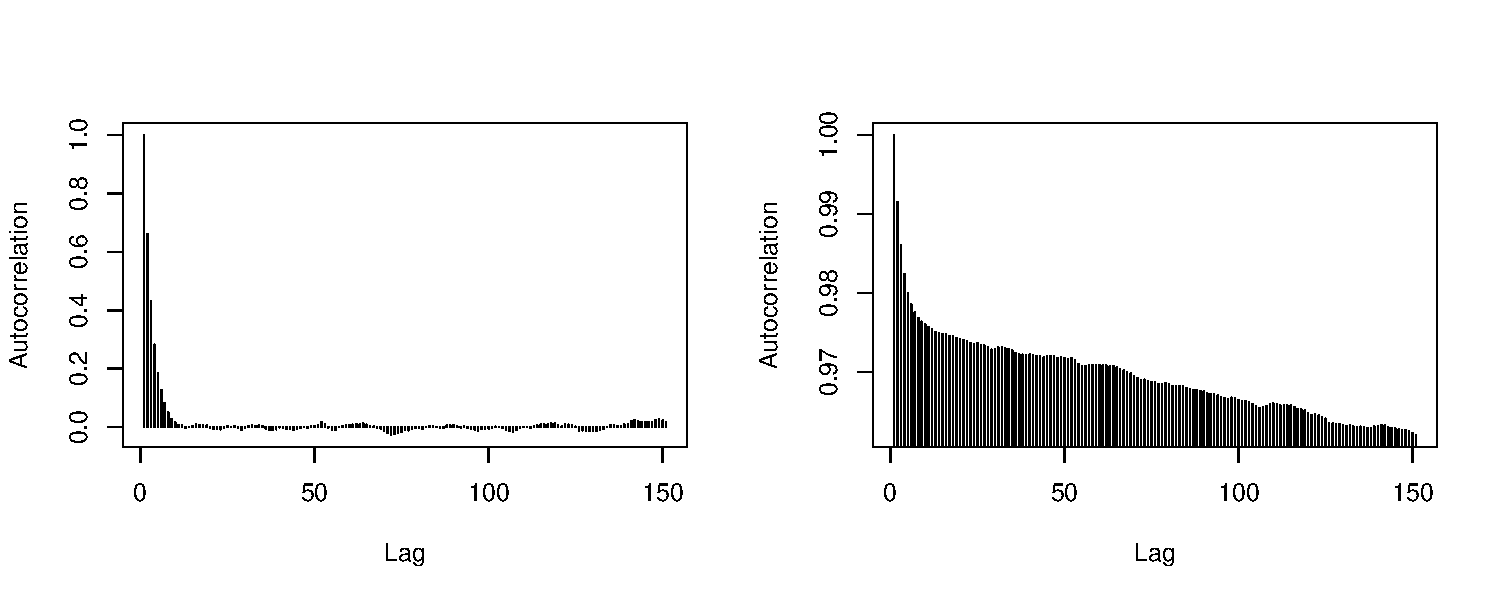
\includegraphics[width=.9\linewidth]{plots/gaussian-acf_n1e4.pdf}
   \caption{$n = 10^4$}
   \label{subfig:gauss-acf-1e4}
 \end{subfigure}\\
 \begin{subfigure}{\textwidth}
   \centering
   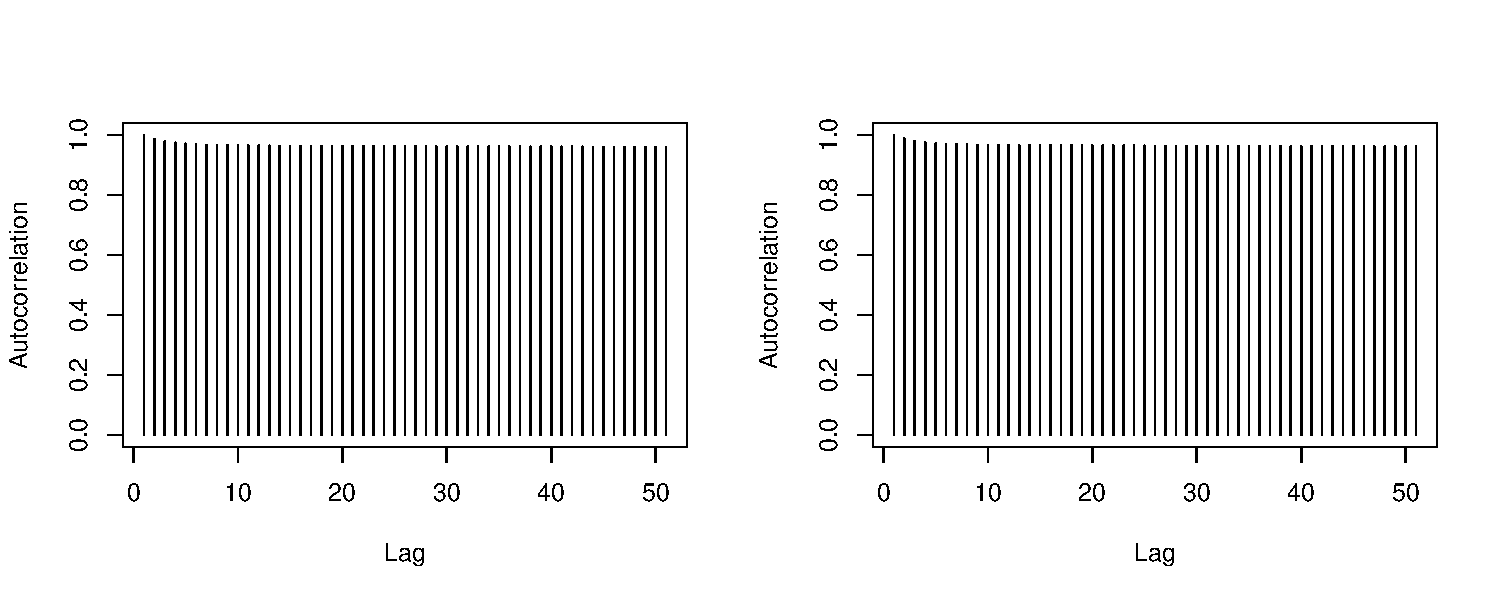
\includegraphics[width=.9\linewidth]{plots/gaussian-acf_n1e5.pdf} 
   \caption{$n = 10^5$}
   \label{subfig:gauss-acf-1e5}
 \end{subfigure}
 \caption{Autocorrelation plot for locally-centered ACF (left) and globally centered ACF (right) averaged over all chains. (a) $n = 10^4$, not converged yet; (b) $n =  10^5$, converged}
 \label{fig:gauss:acf}
\end{figure}
\end{example}



\section{Globally-centered autocovariance} \label{sec:G-ACF}

 Suppose we have $m$ replications of Markov chains for same target distribution and $\{X_{st}; \; t \in \mathbb{Z}\}$ denote the $s^{th}$ Markov chain. Let the sample mean of $s^{th}$ Markov chain be denoted by $\bar{X}_s$ and the global mean by $\bar{\bar{X}} = \sum_{s = 1}^{m}\bar{X}_s/m$. The global mean provides a better estimate for the expectation value when the number of simulation per chain are not sufficient for the convergence to kick in. The globally-centered autocovariance function (G-ACF) for the $s^{th}$ Markov chain is given by:
%
\[
\hat{\Gamma}_{G,s}(k) = \dfrac{1}{n} \sum_{t=1}^{n-k}(X_{st}-\bar{\bar{X}})(X_{s(t+k)}-\bar{\bar{X}})^T
\]

If the starting points of these parallel Markov chains are sufficiently dispersed, G-ACF provides more realistic estimation of lag covariances. \cite{priestley1981spectral} shows that the empirical estimator in Equation \ref{eq:empirical_acf} is biased with the main bias term equal to $\abs{k}\Gamma(k)/n$, ignoring the small order terms arising due to estimation of $\mu$. An unbiased estimator with a divisor of $n - \abs{k}$ instead of $n$ exists, say $\Gamma^*(k)$. Nevertheless, the biased estimator is preferred for its lower mean square error (\cite{priestley1981spectral}). For a small $k$ relative to $n$, the two estimators are almost the same. However, for larger relative $k$ the variance of $\hat{\Gamma}(k)$ compensates for larger bias rendering a smaller mean square error than $\Gamma^*(k)$. 


% \subsection{Theoretical results} % (fold)
% \label{sub:theoretical_results}

% subsection theoretical_results (end)

The bias for G-ACF is similar to the bias of sample autocovariance estimator in case of single chain except for a few small order terms that shall be later addressed in theorem \ref{th:G-_expec}. Before getting to the bias results for $\hat{\Gamma}_{RAV}(k)$ for any lag $k$, we introduce an additional notation. For $q \geq 1$, we define
\[
\Phi^{(q)} = \sum\limits_{-\infty}^{\infty}\abs{k}^q \|\Gamma(k)\|
\]
We denote $\Phi^{(1)} \textrm{ by } \Phi$. 

The proof of the following theorem is available in Appendix~\ref{appendix:bias}.
\begin{theorem} \label{th:G-_expec} Under stationarity,
\[
   \mathbb{E} \left[\hat{\Gamma}_{G,s}(k) \right] = \left(1- \dfrac{|k|}{n}\right) \left(\Gamma(k) - \dfrac{\Sigma}{mn} - \dfrac{\Phi}{mn^2}\right)  + o \left(n^{-2} \right)\,,
\]
and consequently,
\[
\mathbb{E} \left[\hat{\Gamma}_{G,s}(k) - \hat{\Gamma}(k)_s \right] = \dfrac{\abs{k}}{n}\left(1 - \dfrac{1}{m}\right)\left(\dfrac{\Sigma}{n} + \dfrac{\Phi}{n^2}\right) + o\left(n^{-2} \right)\,. 
\]
   % \[
   % \mathbb{E} \left[\hat{\Gamma}_{G}(k) \right] = \left(1- \dfrac{|k|}{n}\right)\left(\Gamma(k) - \dfrac{\Sigma}{mn} - \dfrac{\Phi}{mn^2}\right)  + \dfrac{2(m-1)}{m}\dfrac{\abs{k}}{n^2} \left(\Sigma - \sum_{h=0}^{n-1}\Gamma(h)\right) + o(n^{-2})
   % \]
\end{theorem}

% \begin{proof}
%  The estimator for autocovariance with divisor $n$ is suggested by \cite{parzen1961approach} for its lesser mean square error despite having greater bias than the unbiased estimator with an $n - \abs{k}$ divisor. 
%  We know that $\hat{\Gamma}_s(k)$ is asymptotically unbiased with a $o(1)$ bias term that remains fixed for any $k$. The bias term is given by \cite{priestley1981spectral} as 
 
%  \begin{equation} \label{eq:priestly}
%      \mathbb{E}[\hat{\Gamma}(k)] = \left(1- \dfrac{\abs{k}}{n}\right)\left(\Gamma(k) - \Var{(\bar{X})}
%  \right)
%  \end{equation}
 
% By proposition 1 in \cite{song1995optimal} 
% \begin{equation} \label{eq:song}
% \Var(\bar{X}) = \dfrac{\Sigma}{n} + \dfrac{\Phi}{n^2} + o(n^{-2})
% \end{equation}

% As a consequence, if $\Var(\bar{X})$ is finite, then $\Var(\bar{X}) \to 0 \textrm{ as } n \to \infty$. We can break $\hat{\Gamma}_{G-}$ into four parts for all $k \geq 1$ as:
%  \[
%  \hat{\Gamma}_{G} =  \dfrac{1}{m}\sum_{s=1}^{m}\hat{\Gamma}_s(k) - \dfrac{1}{mn}\sum_{s=1}^{m}\sum_{t=1}^{|k|}A_{st}^T - \dfrac{1}{mn}\sum_{s=1}^{m}\sum_{t=n-|k|+1}^{n}A_{st} + \dfrac{n-|k|}{mn}\sum_{s=1}^{m}(\bar{X}_s - \bar{\bar{X}})(\bar{X}_s - \bar{\bar{X}})^T\,,
%  \]
% %
% where $A_{st} = (X_{st}-\bar{X}_s)(\bar{X}_s - \bar{\bar{X}})^T$\\
% The expectation value of the first term is given by equation \ref{eq:priestly} and \ref{eq:song} while the other three terms contribute $o(1)$ terms. The complete proof evaluating the expectation values of last three terms can be found in Appendix subsection \ref{appendix:bias}.
% \end{proof}

% \begin{remark} \label{rmrk:exp_G-f_minus_acf}
% Using theorem \ref{th:G_expec} and equation \ref{eq:priestly},
% \[
% \mathbb{E} \left[\hat{\Gamma}_{G}(k) - \hat{\Gamma}(k) \right] = \dfrac{\abs{k}}{n}\left(1 - \dfrac{1}{m}\right)\left(\dfrac{\Sigma}{n} + \dfrac{\Phi}{n^2}\right) + \dfrac{2(m-1)}{m}\dfrac{\abs{k}}{n^2} \left(\Sigma - \sum_{h=0}^{n-1}\Gamma(h)\right) + o(n^{-2})
% \]
% We know that the sample autocovariance $\hat{\Gamma}(k)$ underestimates the truth due to a negative bias of $\abs{k}\Gamma(k)/n$ for finite $n$. However, in practice, it is preferred to overestimate the autocovariance for finite $n$ than to underestimate it in order to have a more realistic idea about the correlation in a Markov chain at a particular lag.  Note that the RHS in the above expression is positive. As a consequence, G-ACF will counter this negative bias and give more reliable estimates for ACF. 

% \end{remark}


When $m = 1$, $\hat{\Gamma}_G(k)$ corresponds to $\hat{\Gamma}(k)$, the expectation of which can be found in \cite{priestley1981spectral}. Theorem~\ref{th:G-_expec} implies that the globally-centered autocovariances are asymptotically unbiased and exhibit reduced bias in finite samples compared to locally-centered autocovariances. The consequences of this are particularly pertinent for the diagonals of $\Gamma$. Special interest is also in the lag-0 autocovariance, that is, the variance of the target distribution. 

\begin{corollary} \label{cor:lag0_expectation}
\[
\mathbb{E} \left[\hat{\Gamma}_{G}(0) \right] = \Gamma(0) + \dfrac{\Sigma}{mn} + \dfrac{\Phi}{mn^2} + o(n^{-2})
\]
\end{corollary}

\subsection{Autocorrelation} % (fold)
\label{sub:autocorrelation}

% subsection autocorrelation (end)
For any component $i$, the autocorrelation is
\[
\rho^{(i)}(k) = \dfrac{\Gamma^{(i)}(k)}{\Gamma^{(i)}(0)}\,,
\]
and is particularly useful for visualizing the serial correlation in components of the Markov chain. The typical estimate of the autocorrelation is constructed from  locally-centered autocovariance estimates which as was demonstrated in Section~\ref{sec:intro} can significantly underestimate the autocorrelation. 
\[
\hat{\rho}_{G,s}^{(i)}(k) = \dfrac{ \hat{\Gamma}^{(i)}_{G,s} (k)}{\hat{\Gamma}^{(i)}_{G,s} (0)}
\]
{\color{blue} Add more about autocorrelation}

% \begin{proof}
%  The proof is in Appendix subsection \ref{appendix:bias}.
% \end{proof}


\section{Variance Estimators for multiple Markov chains} \label{sec:variance_est}

{\color{blue}Dootika: this section here needs to be much tighter in its presentation. We will need to remember that the paper is no longer about the SV estimators but about autocorrelations. So will have to present the discussion similarly. }


  Suppose $F$ is the target distribution on support $\chi \subseteq \mathbb{R}^d$. For $g:\chi \longrightarrow \mathbb{R}^p$ be an F-integrable function. We are interested in
%
\[
\mu_g = \mathbb{E}_F[g(X)] = \int_{\chi}g(x)F(dx)
\]
 
Let $\{X_{t}\}_{t \geq 1}$ denote the Harris ergodic (aperiodic, F-irreducible, and positive Harris recurrent) Markov chain having invariant distribution $F$. We will use the following Monte Carlo estimator in order to estimate $\mu$
%
\[
\hat{\mu}_s = \dfrac{1}{n}\sum_{i = 1}^{n} g(X_{si}) \xrightarrow{a.s.} \mu \textrm{ as } n \to \infty
\]

We are interested in Markov chain average and therefore, throughout this paper, we will deal with the function $g(X) = X$. To assess the reliability of our simulations, we are interested in Monte Carlo error, i.e. $\bar{\bar{X}} - \mu$. The sampling distribution for Monte Carlo error is available via Markov chain CLT (\cite{jones2004markov}) if there exists a positive definite matrix $\Sigma$ such that
%
\[
\sqrt{n}(\bar{X}_s-\mu) \xrightarrow{d} N(0,\Sigma)
\]

 It is important to construct an estimator for $\Sigma$ which is very close to underlying reality. There are many techniques for estimating $\Sigma$ like batch means (BM), overlapping bath means (OBM), and spectral variance estimator (SVE). Due to its nice statistical properties and heavy dependence on autocovariance, we will only focus on SVE in this paper. SVE involves a truncated and weighted sum of autocovariances. We will give theoretical as well as experimental results for the version of SVE that uses our globally centered autocovariances. We call this globally-centered SVE (G-SVE). 
 





Given m parallel Markov chains, we have $m$ i.i.d. samples of $\bar{X}_s$, $s \in \{1,..., m\}$. The Markov Chain standard error (MCSE) is given by $\Sigma/mn$. We are interested in consistent estimates of $\Sigma$ for two reasons. Firstly, to construct asymptotically valid confidence intervals and secondly, to determine when to stop the simulations. For this purpose, we use the class of Multivariate Spectral Variance Estimators (MSVE). The most common practice would be to combine the spectral variance estimates from $m$ chains by averaging over them. We call this technique average spectral variance estimator and denote it by $\hat{\Sigma}_A$). We propose using a globally-centered spectral variance estimator (G-SVE) wherein we use G-ACF to estimate the autocovariance. Strong consistency for MSVE has been addressed by \cite{vats:fleg:jon:2018}. Bias and variance calculations for a variant of SVE with known mean is done by \cite{hannan2009multiple}. In this paper, we will address the asymptotic properties (strong consistency), bias and variance calculations for G-SVE. 

\subsection{Globally-centered spectral variance estimators} % (fold)
\label{sub:globally_centered_spectral_variance_estimators}

% subsection globally_centered_spectral_variance_estimators (end)

Recall from Equation \ref{eq:empirical_acf} that $\hat{\Gamma}(k)$ is the empirical autocovariance function given by 

\begin{equation}
    \hat{\Gamma}(k) = \dfrac{1}{n}\sum_{t=1}^{n-\abs{k}}(X_t - \bar{X})(X_{t + \abs{k}} - \bar{X})^T
\end{equation}


The spectral variance estimator is the weighted and truncated sum of lag-k autocovariances, given by:

\begin{equation} \label{eq:sve}
    \hat{\Sigma}_{SV} = \sum_{k=-b_n+1}^{b_n-1}w\left(\dfrac{k}{b_n}\right)\hat{\Gamma}_n(k)
\end{equation}

where $w(.)$ is the lag window and $b_n$ is the truncation point. Consider $m$ Markov chains where $\hat{\Gamma}_s(k)$, $\hat{\Gamma}_{G,s}(k)$ and $\hat{\Sigma}_{S, s}$ are the lag-$k$ empirical ACF, G-ACF, and SVE respectively for $s^{th}$ Markov chain, $s\in {1,...,m}$. We construct the globally-centered SVE estimator $\hat{\Sigma}_{G}$ using the globally-centered ACF. Consider, 
%
\begin{align*}
    \hat{\Sigma}_{G,s} &= \sum_{k=-b_n+1}^{b_n-1}w\left(\dfrac{k}{b_n}\right)\hat{\Gamma}_{G,s}(k)
\end{align*}
\[
\hat{\Sigma}_{G} =  \dfrac{1}{m}\sum_{s=1}^{m}\hat{\Sigma}_{G,s}
\]


\subsubsection{Theoretical results} \label{sec:G-SVE}

The G-SVE estimator centers the data around the global mean. We are interested in proving the strong consistency, finding the bias and variance of G-SVE. 

\begin{ass}[Strong Invariance Principle (SIP)] \label{ass:sip}
    We assume the SIP holds for the Markov chain. Here $\{X_t\}_{t\geq 1}$ is the stochastic process that follows SIP with mean $\mu$. Let $\|.\|$ denote the Euclidean norm. Through SIP, there exists a $p \times p$ lower triangular matrix L, an increasing function $\psi$ on the integers, a finite random variable D, and a  sufficiently rich probability space such that, with probability 1, \\
  $$\left\|\sum_{t=1}^{n}X_t - n\mu - LB(n)\right\| < D\psi(n)$$
  
  Let $\{B(n)\}_{n\geq 0}$ denotes a standard p-dim Brownian motion and $B^{(i)}$ denotes its $i^{th}$ component. As shown in the results \cite{kuelbs1980almost}, SIP will hold for $\psi(n) = n^{1/2 - \lambda, \; \lambda > 0}$ for Markov chains commonly encountered in MCMC settings. We know that $\psi(n)$ is an inherent property of the stochastic process that satisfies the CLT. This implies that $\psi(n)$ is at least $o(\sqrt{n})$. Using Law of Iterative Logarithms (LIL), a tighter bound for $\psi(n)$ is given by \cite{stra:1964} as $\mathcal{O}(\sqrt{n\log \log n})$.
\end{ass}


\begin{ass} \label{ass:sve_consis} We assume that all the conditions given by \cite{vats:fleg:jon:2018} for strong consistency of the spectral variance estimator hold true. As a consequence, 
\[
\hat{\Sigma}_{S,s} \xrightarrow{a.s.} \Sigma \textrm{ as } n \to \infty \;\; \forall s \in \{1,..., m\}
\]
\end{ass}




\begin{theorem}
\label{th:consistency}
 Let the Assumptions \ref{ass:sip},\ref{ass:sve_consis} hold and $n^{-1}{b_n \log \log n} \to 0 \textrm{ as } n \to \infty$, then $\hat{\Sigma}_{G} \to \Sigma$ with probability 1, as $n \to \infty$.
\end{theorem} 

% \begin{proof}
% We complete the proof by showing that $\hat{\Sigma}_{G}^{ij} - \tilde{\Sigma}^{ij}$ converges to 0 almost surely for all $i,j \in \{1,...,p\}$ and $\tilde{\Sigma}^{ij} \to \Sigma^{ij}$ with probability 1 as $n \to \infty$. We will show that 

% \[
% \hat{\Sigma}_{G-SVE}^{ij} - \tilde{\Sigma}^{ij} = g_1(n)D^2 + g_2(n)D + g_3(n)
% \]
% where $D$ is the finite random variable associated with SIP. We will show that
% \begin{align*}
%     g_1(n) &= (4+C_1)\dfrac{b_n \psi^2(n)}{n^2} - 4\dfrac{\psi^2(n)}{n^2}\\
%     g_2(n) &= 2\sqrt{2}\|L\|p^{1/2}(1+\epsilon)\left[(4+C_1)\dfrac{b_n\psi(n)\sqrt{n\log \log n}}{n^2} - 4\dfrac{\psi(n)\sqrt{n\log \log n}}{n^2}\right]\\
%     g_3(n) &= \|L\|^2 p (1+\epsilon)^2\left[(4+C_1)\dfrac{b_n \log\log n}{n} - 4 \dfrac{\log \log n}{n}\right]
% \end{align*}

% Using $\psi(n) = \mathcal{O}(\sqrt{n \log \log n}),\; b_n = o(n), \textrm{ and } b_n \log \log n = o(n)$, we can finally we prove that $g_1(n), g_2(n), g_3(n) \to 0$ with probability 1, as $n \to \infty$. The proof is in Appendix subsection \ref{appendix:strong_consis}
% \end{proof}

We are interested in the finding the bias for G-SVE estimator as a function of $n$. The proof below applies to all the important range of lag windows $w(x)$; where $w(x)$ is a continuous, even fnction with $w(0)=1, \abs{w(x)} < c$, and $\int_{-\infty}^{\infty}w^2(x)dx < \infty$. Define
%
\[
W_n = \dfrac{1}{2\pi}\sum_{k=-b_n+1}^{b_n-1}w\left(\dfrac{k}{b_n}\right).
\]

We have $W_n < \infty$ for all the important lag windows.

\begin{ass} \label{ass:bias}
    Let $\Gamma_s(k)$ be the lag-k autocovariance for $s^{th}$ Markov chain and $w(x)$ be the lag window. We assume that there exists a $q \geq 0$ such that for all $s$
    \begin{enumerate} [a.]
        \item $\sum\limits_{-\infty}^{\infty}\abs{k}^q \|\Gamma_s(k)\| < \infty$
        \item $\lim _{x \to 0}\dfrac{1 - w(x)}{\abs{x}^q} = k_q < \infty$
        \item $\dfrac{b_n^q}{n} \to 0$ as $n \to \infty$
    \end{enumerate}
    
    If $k_q$ is finite for some $q_o$, then it is zero for $q < q_0$. $q$ is taken to be the largest number satisfying the first two conditions above.
\end{ass}


\begin{theorem}\label{th:G-SVE_bias}
The limiting bias of replicated spectral variance is given by:
\[
 \lim_{n \to \infty}b_n^q\mathbb{E} \left[\hat{\Sigma}_{G} - \Sigma \right] = -k_q\Phi^{(q)}
 \]
\end{theorem}

% \begin{proof}
% \[
% \mathbb{E} \left[\hat{\Sigma}_{G} - \Sigma \right] = \sum_{k=-b_n+1}^{b_n-1} w\left(\dfrac{|k|}{b_n}\right)\mathbb{E} \left[\hat{\Gamma}_{G}(k) \right] - \sum_{k=-\infty}^{\infty}\Gamma(k)
% \]

% Using theorem \ref{th:G-ACF_expec}, we can write the expectation of $\hat{\Gamma}_{G}$ as  a sum of equation \ref{eq:priestly} and some small order terms.
% The proof is given in the Appendix subsection \ref{appendix:bias}.
% \end{proof}


\begin{ass} \label{ass:variance_cal}
Let $\{X_{st}\}_{t \geq 1}$ be the $s^{th}$ Markov chain for which SIP holds. 
\begin{enumerate}[a.]
    \item $\E[D^4] < \infty$ where D is a finite random variable associated with the SIP
    \item $\E[X^4] < \infty$ where $\{X\}$ is the stochastic process
\end{enumerate}
\end{ass}


\begin{theorem} \label{th:G-SVE_variance}
 If Assumption \ref{ass:variance_cal} holds, $b_n^{-1}{n}\Var \left(\hat{\Sigma}_{G}^{ij} \right) = [\Sigma_{ii}\Sigma_{jj} + \Sigma_{ij}^2]\int_{-\infty}^{\infty}w(x)^2dx  + o(1)$.
\end{theorem}



% \begin{proof}
% Recall that $\tilde{\Sigma}$ is the averaged pseudo spectral variance estimator which uses the unobserved mean. Further, let $\tilde{\Sigma}^{ij}$ be the $(i,j)^{th}$ element of this matrix. We will prove that the variance of $\hat{\Sigma}_{G} \textrm{ and } \tilde{\Sigma}$ are equivalent for large sample sizes. The proof is in Appendix subsection \ref{appendix:variance}
% \end{proof}

\subsubsection{Fast implementation} % (fold)
\label{ssub:fast_implementation}

The multivariate spectral variance estimator (MSVE) despite having good statistical properties poses application limitations due to slow computation and high storage demands. Observe from equation \ref{eq:empirical_acf} and \ref{eq:sve}, the computation of spectral variance estimator has a complexity of $\mathcal{O}(b_n n p)$ where $n$ is the MCMC sample size, $p$ is the dimensionality and $b_n$ is the truncation point. To overcome this limitation for our experimental purposes, we used a fast Fourier transform based algorithm presented by \cite{heberle2017fast} for calculating the alternate formulation of MSVE given by Kyriakoulis (2005).\\

Suppose $\{X_t\}_{t=1}^n$ is the Markov chain of $n$ samples where $\overline{X}_n = \dfrac{1}{n}\sum_{t=1}^{n}X_t$ is the MCMC average. Let $w_k$ denote the lag-window at lag-k, i.e. $w_k = w_n(k/b_n)$. The alternate formulation for MSVE is given by
%
\[
    \hat{\Sigma}_{SV} = \dfrac{1}{n}A^T T(w) A, \qquad \textrm{ where } A = \begin{pmatrix}
    X_1 - \overline{X}_n  & \dots & X_n - \overline{X}_n
\end{pmatrix}^T
\]

and $T(w)$ is the $n \times n$ Toeplitz matrix of weights with the first column being $(1 ~ w_1 ~ w_2 ~ \dots, ~ w_{n-1})^T$
%  $w = 
% \begin{pmatrix}
%     1 & w_1 & w_2 & \dots w_{n-1}
% \end{pmatrix}^T$.
$T(w)$ is an $n \times n$ matrix which can be difficult to store. Therefore, \cite{heberle2017fast} computed $T(w)A$ directly using an FFT based algorithm. The algorithm requires embedding $T(w)$ in a $2n \times 2n$ circulation matrix $C(w^*)$. We write the spectral decomposition of $C(w^*)$ as $V\Lambda V^*$. A is extrapolated into a $2n \times p$ matrix $A^*$ such that
\[
    \hat{\Sigma}_{SV} = \dfrac{1}{n} A^T T(w) A = \dfrac{1}{n} A^T (C(w^*) A^*)_{1:n, :} = \dfrac{1}{n} A^T (V \Lambda V^* A^*)_{1:n, :}).
\]
The complete algorithm is as follows


\begin{algorithm}[htbp]
\DontPrintSemicolon
\SetAlgoLined
Construct $C(w^*) \textrm{ and } A^*$ from the MCMC samples.\\ Compute the DFT of the first column of $C(w^*)$. This gives the eigenvalues of $C(w^*)$.\;
\For{$j = 1, 2, ..., p$}    
    { 
    Calculate $V^*A_j^*$ by FFT of $A_j$\;
    Multiply the $i^{th}$ entry of the vector $V^* A_j^*$ with the eigenvalue $\lambda_i$ for all $i = 1, 2, ..., 2n$ in order to construct $\Lambda V^* A_j^*$.\;
    Determine $C(w^*)A^* = V \Lambda V^* A_j^*$ by inverse FFT of $\Lambda V^* A_j^*$.\;
    }
 Select the first $n$ rows of $C(w^*)A^*$ to form $T(w)A$.\;
 Premultiply by $A^T$ and divide by $n$.
 \caption{Herberle's Algorithm}
\end{algorithm}

The algorithm has been implemented in the \texttt{R} package \texttt{mcmcse} for fast implementation of spectral variance estimators. We do a slight variation in the alternate formulation of SVE proposed by Kyriakoulis (2005) by centering the chain $\{X_{st}; \; t \in \mathbb{Z}\}$ around $\overline{\overline{X}}$ instead of $\overline{X}_s$ for all $s \in \{1, ..., m\}$. Herberle's algorithm is then applied on the formulation

\[
\hat{\Sigma}_{S,s} = \dfrac{1}{n}B^T T(w) B \qquad \textrm{ where } B = 
\begin{pmatrix}
    X_{s1} - \overline{\overline{X}} \; \dots \; X_{sn} - \overline{\overline{X}}
\end{pmatrix}^T
\].

% subsubsection fast_implementation (end)

\section{Effective sample size} \label{sec:ess}

Estimating the MCSE is crucial for determining when to terminate the simulations. The existing stopping rules rely on the strong consistency of the estimator of $\Sigma$. The determinant of Monte Carlo standard error is called generalized variance in  \cite{wilks1932certain} and gives a metric for volume of confidence interval. 

We will use the multivariate effective sample size (m-ESS) by \cite{vats2019multivariate} to understand the effectiveness of simulations so far. m-ESS requires a strongly consistent estimator of $\Sigma$. G-SVE better captures the MCSE by considering the global sample mean across the Markov chains; which might otherwise get lost when considering a single localized slowly mixing Markov chain. We therefore define our ESS estimator as

\[
\text{ESS} = mn\left(\dfrac{\abs{\Lambda_{mn}}}{\abs{\hat{\Sigma}_{G}}}\right)^{1/p}
\]

where $\Lambda_{mn}$ is the sample covariance of $mn$ samples. When there is no correlation in Markov chain $\hat{\Sigma}_{G} = \Lambda_{mn}$ and therefore, ESS = $n$. 

\section{Examples} \label{sec:examples}

There are only a handful of stochastic processes where the true autocovariance and $\Sigma$ are known. To compare the estimators when the truth is known, we use a slowly mixing vector autoregressive process of order 1 (VAR(1)). A more promising advantage of our estimators is observed when the target distribution is multi-modal. For this purpose we use a bivariate bi-modal probability distribution introduced by \cite{gelman1991note} in section \ref{ex:boomerang}. Through this example, we will also show that in case of nicely mixing Markov chains, these estimators give almost equivalent results. As a consequence, while out replicated version of variance estimator is better in cases where the Markov chains do not explore the entire sample space in finite time, it is harmless to be used in cases where they do. Lastly, we consider a real-life example of finding unknown locations of sensors using noisy distance data in section \ref{ex:sensor_post}. The posterior distribution is this case is marginally bimodal in all dimensions. All the examples have been selected to display some kind of \textit{sticky} nature in the Markov chains. In such scenario, we successfully show that our globally-centered estimators yield better results as compared to the classical autocovariance function, spectral variance estimator, and effective sample size.


\subsection{Vector Autoregressive Process} \label{ex:var}

We examine the vector autoregressive process of order 1 (VAR(1)) where the true autocovariance in known in closed form. Consider a p-dimensional VAR(1) process $\{X_t\}_{t \geq 1}$ such that
%
\[
X_t = \Phi X_{t-1} + \epsilon_t
\]

where $X_t \in \mathbb{R}^p$, $\Phi $ is a $p \times p $ matrix, $ \epsilon_t \overset{i.i.d.}{\sim} N(0, \Omega)$, and $\Omega$ is a positive definite $p \times p$ matrix. The invariant distribution for this Markov chain is $N(0, \Psi)$ where $\Vec{\Psi} = (I_{p^2} - \Phi \otimes \Phi)\Vec{\Omega}$. The lag-k autocovariance can be calculated easily for $k >0$ as
%
\begin{align*}
    \Gamma(k) &= \Phi^k\Psi\\
    \Gamma(-k) &= \Psi(\Phi^T)^k
\end{align*}

The Markov chain is geometrically ergodic when the spectral norm of $\Phi$ is less than 1 (\cite{10.2307/1427459}). The CLT holds for the invariant distribution, therefore, $\Sigma$ exists and is given by
%
\[
\Sigma = (1 - \Phi)^{-1}\Psi + \Psi(1 - \Phi^T)^{-1} - \Psi
\]

Let $\phi_{max}$ be the largest absolute eigenvalue of $\Phi$ such that $\abs{\phi_{max}} < 1$. The larger it is, the slower the Markov chain mixes. For our case, we require a slowly mixing VAR(1) process. We consider a bivariate example with $\phi_{max} = 0.9999$. We run five parallel Markov chains with their starting points evenly distributed about the center of invariant distribution. Figure \ref{subfig:var-sp_500} shows that for the first 500 samples, the chains have not explored the sample space well unlike Figure \ref{subfig:var-sp_50000} with $5\cdot 10^4$ samples.  

% \begin{figure}[h]
%     \centering
%     \begin{subfigure}[h]{0.4\textwidth}
%          \centering
%          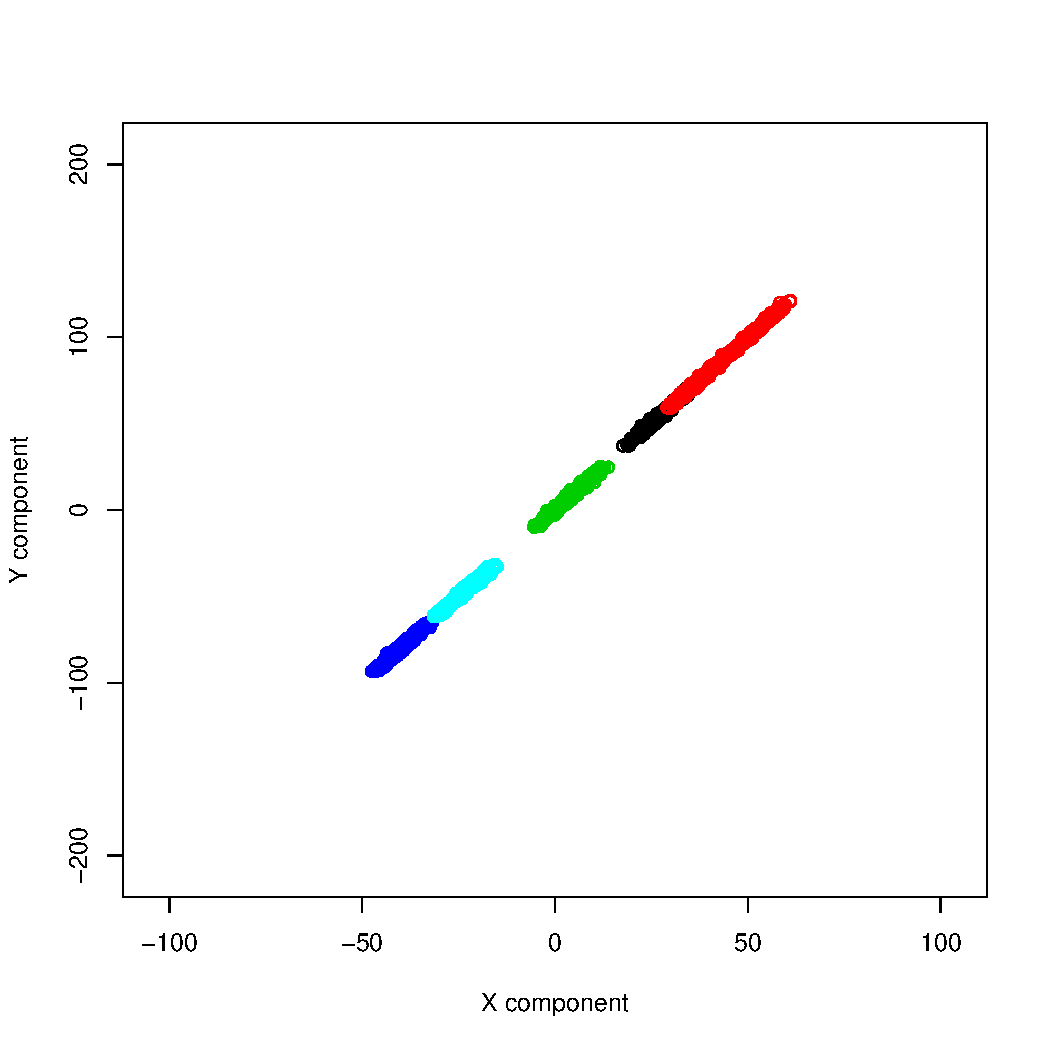
\includegraphics[width=\textwidth]{plots/scatter_plot_500.pdf}
%          \caption{$n = 500$}
%          \label{subfig:var-sp_500}
%      \end{subfigure}
%      \begin{subfigure}[h]{0.4\textwidth}
%          \centering
%          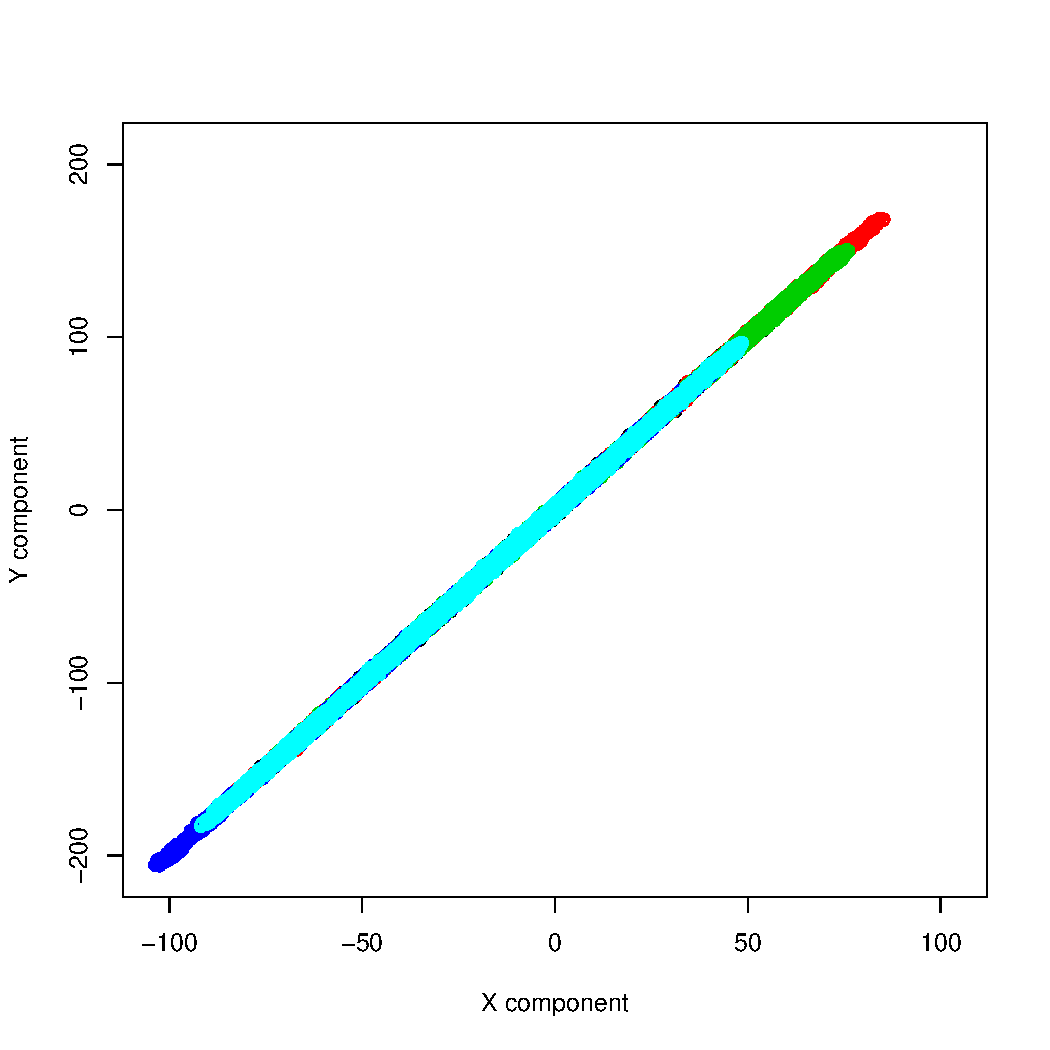
\includegraphics[width=\textwidth]{plots/scatter_plot_50000.pdf}
%          \caption{$n = 5 \times 10^4$}
%          \label{subfig:var-sp_50000}
%      \end{subfigure}
%     \caption{Scatter plot of five Markov chains for different sample sizes.}
%     \label{fig:var-sp}
% \end{figure}

\begin{figure}[htbp]
 \begin{subfigure}{\textwidth}
   \centering
   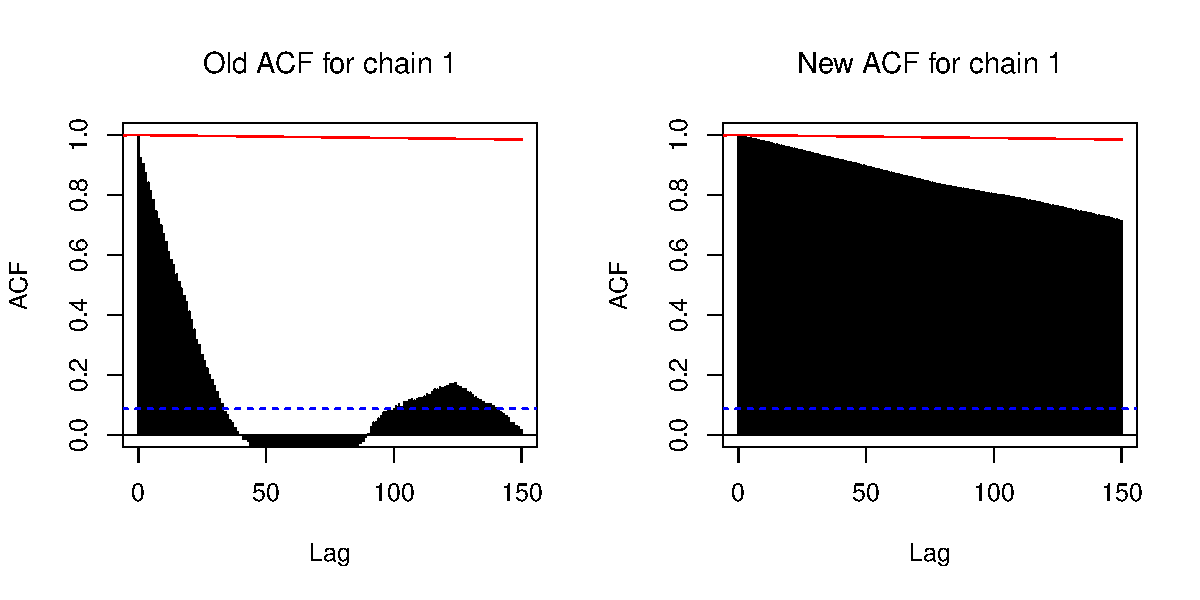
\includegraphics[width=.6\linewidth]{plots/acf,n=500.pdf}
   \caption{$n = 500$}
   \label{subfig:acf-500}
\end{subfigure}\\
\begin{subfigure}{\textwidth}
  \centering
  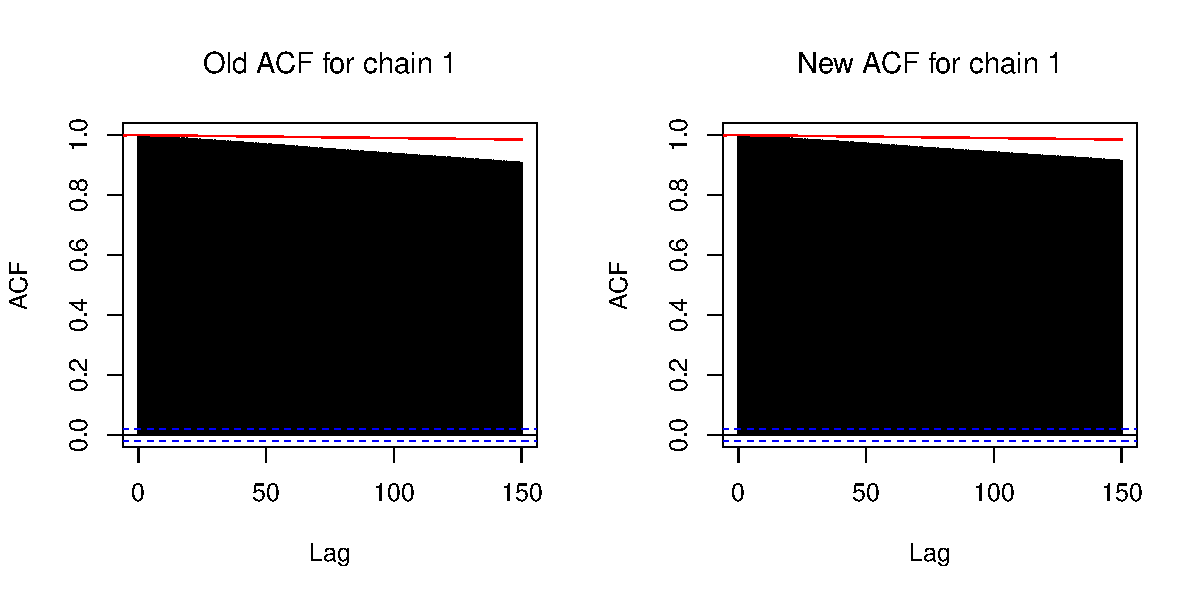
\includegraphics[width=.6\linewidth]{plots/acf,n=10000.pdf} 
  \caption{$n = 10^4$}
  \label{subfig:acf-5e4}
\end{subfigure}
\caption{Autocorrelation plot for ACF and G-ACF for first chain out of two parallel Markov chains. First column corresponds to ACF calculated using arithmetic mean of first Markov chain and the second column corresponds to the one calculated using global mean of two Markov chains.(a): $n = 500$, not converged yet; (b): $n =  10^4$, converged}
\label{fig:var-acf}
\end{figure}


\begin{figure}[htbp]
    \centering
    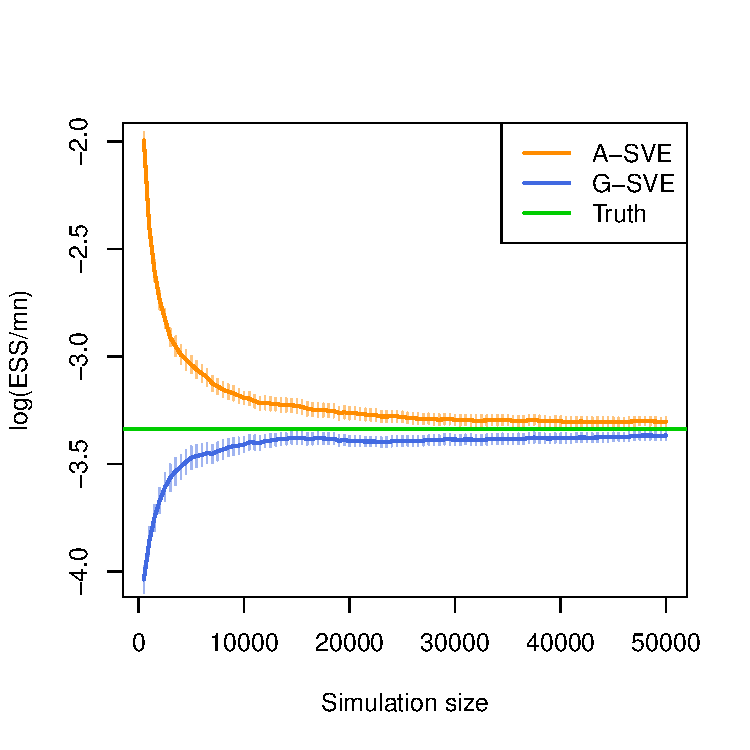
\includegraphics[width = .35\textwidth]{plots/var-ess.pdf}
    \caption{Running plots for $\hat{\text{ESS}}/mn$ calculated using ASV and G-SVE with the truth.}
    \label{fig:var-ess}
\end{figure}


\subsection{Boomerang Distribution} \label{ex:boomerang}

We will use a bivariate bi-modal distribution introduced by \cite{gelman1991note} which has Gaussian conditional distributions in both directions. This allows us to sample parallel Markov chains using the Gibbs sampler. Let $x$ and $y$ be two random variable that are jointly distributed as 
%
\[
f(x, y) \propto \exp\left(-\dfrac{1}{2} \left[Ax^2y^2 + x^2 + y^2 -2Bxy  -2C_1x - 2C_2y  \right]\right)
\]

The conditional distribution of $x$ given $y$ and vice versa is a normal distribution given by:
%
\begin{align*}
    x_1 \mid x_2 &\sim N\left(\dfrac{Bx_2 + C_1}{Ax_2^2 + 1}, \dfrac{1}{Ax_2^2 + 1}\right)\\
    x_2 \mid x_1 &\sim N\left(\dfrac{Bx_1 + C_2}{Ax_1^2 + 1}, \dfrac{1}{Ax_1^2 + 1}\right)
\end{align*}

We use a carefully chosen parameterization of $A = 1,\; B = 3,\; C = 8$ which ensures bimodality for our purpose.  Let $n$ be the number of samples in each chain and $m$ be the number of Markov chain replications. Finding the actual mean of this distribution in closed form is difficult. Therefore, we use numerical integration with fine tuning to calculate it. We sample two parallel Markov chains with well-separated starting values. 

\begin{comment}
\begin{figure}[htbp]
    \centering
    \begin{subfigure}[h]{.4\textwidth}
        \centering
        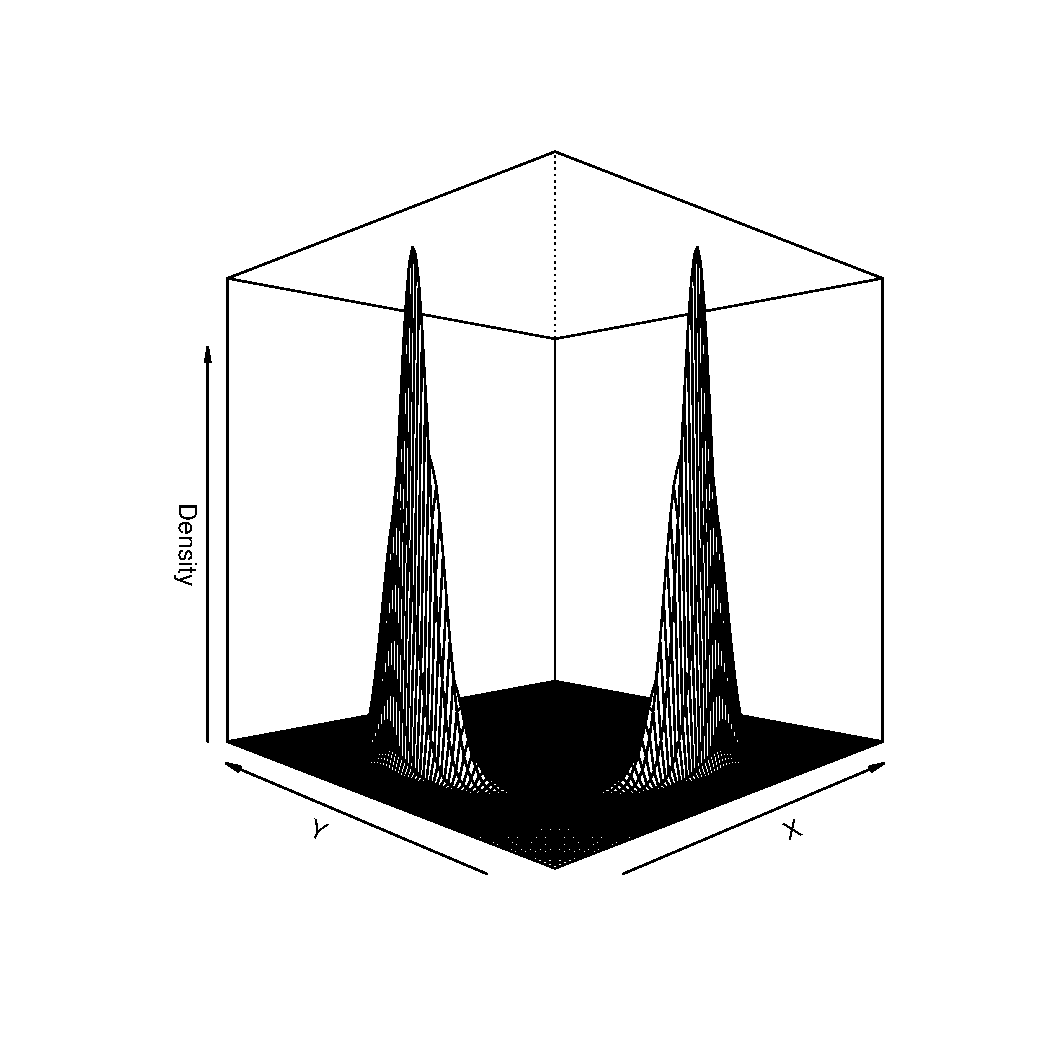
\includegraphics[width = \textwidth]{plots/boom-pers_1_3_8.pdf}
        \caption{$A = 1, B = 3, C = 8$}
        \label{subfig:boom-pers_1_3_8}
    \end{subfigure}
    \begin{subfigure}[h]{.4\textwidth}
        \centering
        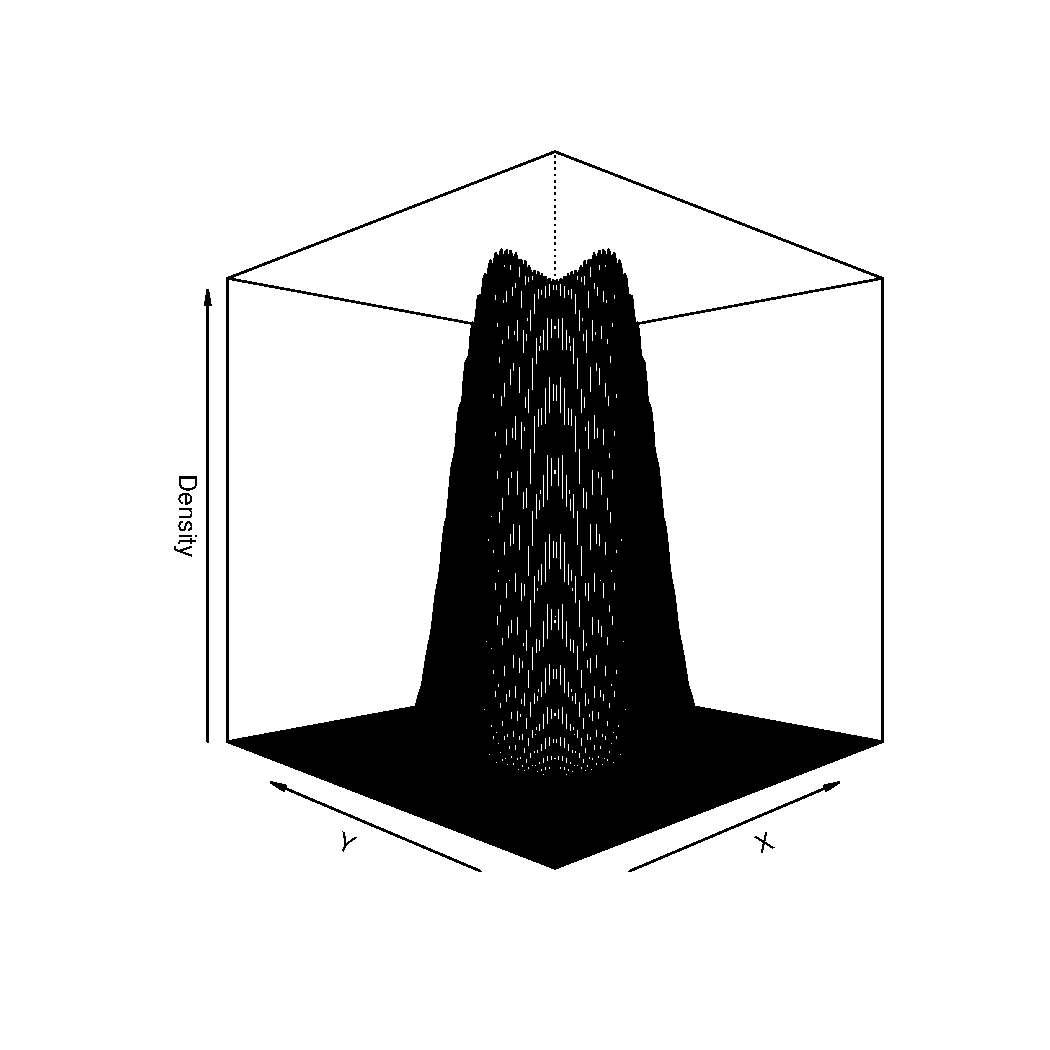
\includegraphics[width = \textwidth]{plots/boom-pers_1_10_7.pdf}
        \caption{$A = 1, B = 10, C = 7$}
        \label{subfig:boom-pers_1_10_7}
    \end{subfigure}
    \caption{Perspective plots of the target distribution for two different parameterizations.}
   \label{fig:3d_plot}
\end{figure}
\end{comment}

\begin{comment}
\begin{figure}[htbp]
    \centering
    \begin{subfigure}[h]{.4\textwidth}
      \centering
      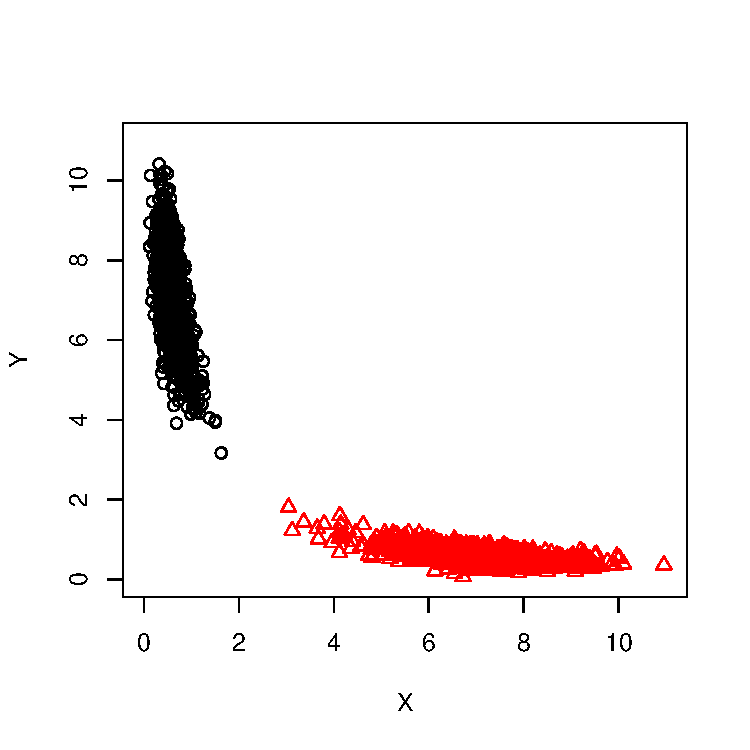
\includegraphics[width = \textwidth]{plots/scatter_n1000.pdf}
      \caption{$n = 1000$}
      \label{subfig:boom-sp_1e3}
    \end{subfigure}
    \begin{subfigure}[h]{.4\textwidth}
      \centering
      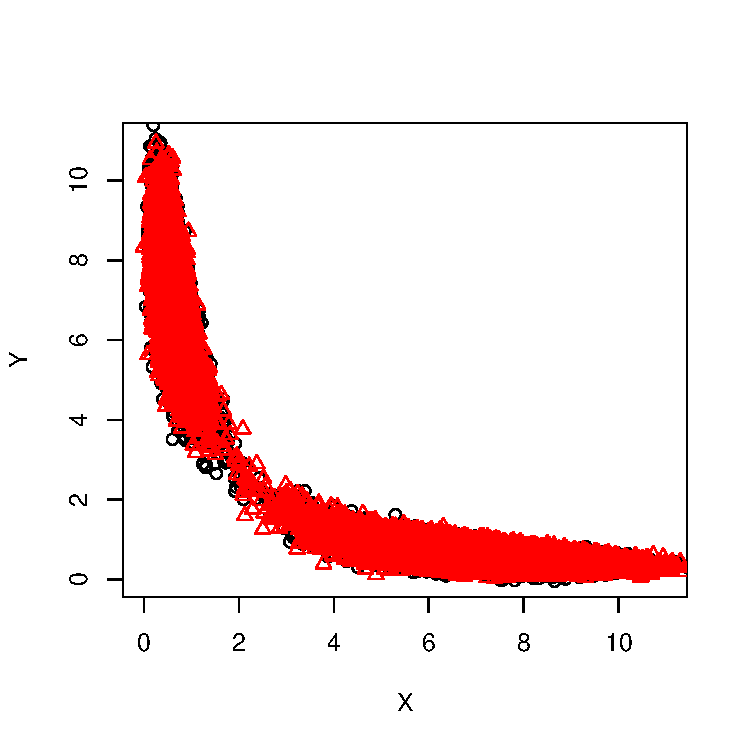
\includegraphics[width = \textwidth]{plots/scatter_n50000.pdf}
      \caption{$n = 50000$}
      \label{boom-sp_1e4}
    \end{subfigure}
    \caption{The scatter plots for two parallel Markov chains. (a): Both the chains are stuck in one of the mode (b): Both the chains have travelled and explored both the modes.}
    \label{fig:boom-sp}
\end{figure}
\end{comment}

%
In Figure \ref{fig:boom-sp}, we demonstrate the ``sticky'' nature of the Markov chains. For the first thousand samples, both the chains are oblivious of the existence of another mode. By ten thousand samples, both the Markov chains have explored the two modes. This property will affect the estimation of ACF from a single chain. In Figure \ref{subfig:boom-acf_1e3}, the ACF is severely underestimated because the first chain has not jumped to the other mode. Whereas, in Figure \ref{subfig:boom-acf_1e4}, both ACF and G-ACF give almost similar results indicating that both modes have been explored by chain-1. 

\begin{figure}[htbp]
    \centering
    \begin{subfigure}[h]{.8\textwidth}
      \centering
      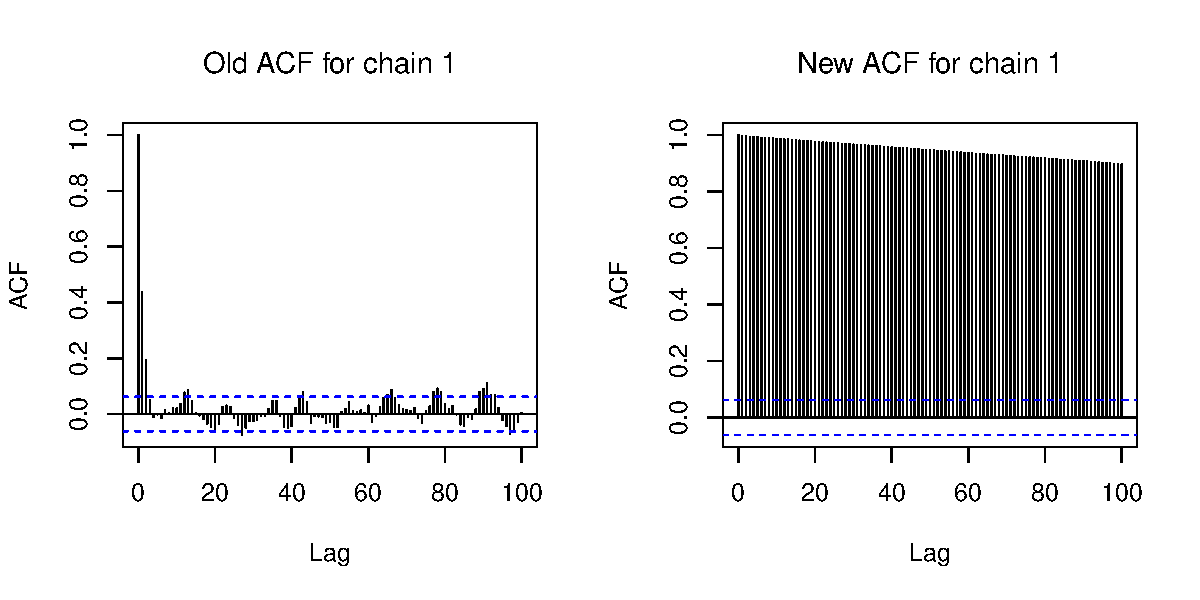
\includegraphics[width = .8\textwidth]{plots/boom-acf,n=1000.pdf}
      \caption{$n = 1000$}
      \label{subfig:boom-acf_1e3}
    \end{subfigure}
    \begin{subfigure}[h]{.8\textwidth}
      \centering
      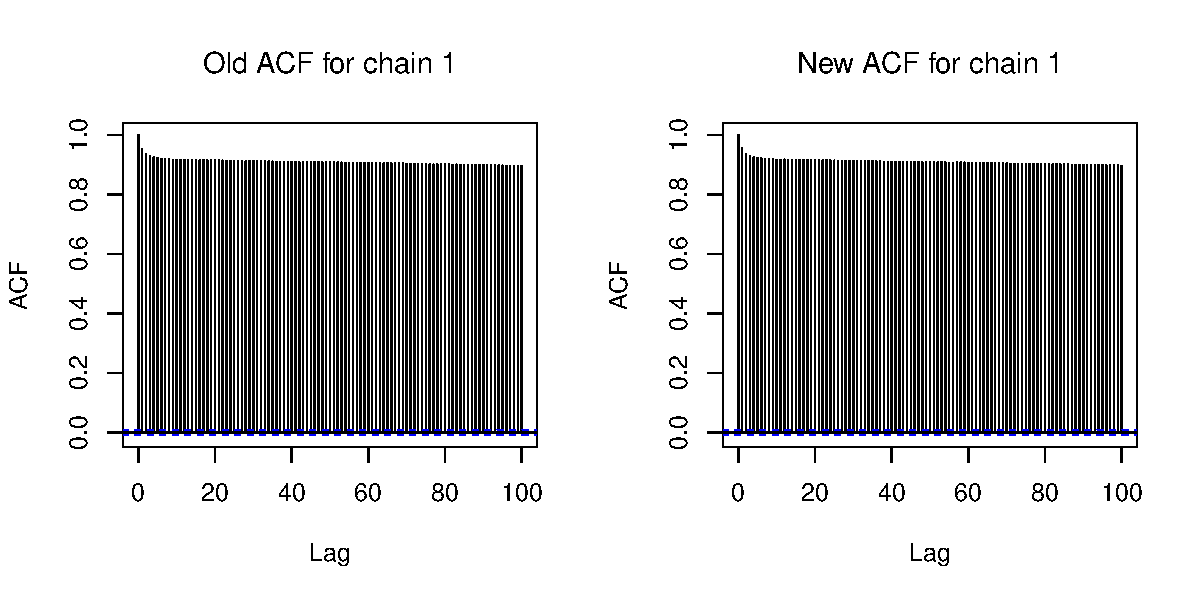
\includegraphics[width = .8\textwidth]{plots/boom-acf,n=50000.pdf}
      \caption{$n = 50000$}
      \label{subfig:boom-acf_1e4}
    \end{subfigure}
    \caption{ACF and G-ACF for component-1 of chain-1 at two different number of Monte Carlo samples. }
    \label{fig:boom-acf}
\end{figure}

We also run five parallel Markov chains with well-separated starting points. In Table \ref{table:boom-coverage_1_3_8}, we give the coverage probabilities for $95 \%$ confidence interval for both the estimator. We can see that the G-SVE gives better coverage probabilities for all the $n$. For smaller sample size, the coverage probability of G-SVE is significantly higher than A-SVE. As the number of samples per chain increases, they start coming closer due to the strong consistency of both the estimators.

\begin{table}[htbp]
\centering
    \begin{tabular}{|c|l|l|l|l|}
    % \toprule
    \hline
        $n$ & \multicolumn{2}{|c|}{$m = 2$} & \multicolumn{2}{|c|}{$m=5$}\\
        \hline
        & ASV & G-SVE & ASV & G-SVE\\
        \hline
        $1000$ & 0.612 & 0.689 & 0.602 & 0.753   \\
        $2000$ & 0.693 & 0.751 & 0.735 & 0.827 \\
        $5000$  & 0.826 & 0.854 & 0.847 & 0.880 \\
        $10000$  & 0.862 & 0.868 & 0.884 & 0.907 \\
        $20000$ & 0.899 & 0.906 & 0.922 & 0.934  \\ \hline
    % \bottomrule
    \end{tabular}
    \caption{Coverage probabilities for parameter values $A = 1,\; B = 3,\; C = 8$. }
    \label{table:boom-coverage_1_3_8}
\end{table}

A good estimate of ESS is crucial to determine when to stop the simulations. We can see in Figure \ref{fig:run_ess} that for the first few thousand samples, A-SVE gives misleadingly higher $\hat{ESS}/mn$ than G-SVE. This can cause us to stop the sampling before the sample space has been explored by the chains. The inferences derived from this chain would then be severely non-informative.

\begin{figure}[htbp]
    \centering
    
    \begin{subfigure}[h]{.3\textwidth}
      \centering
      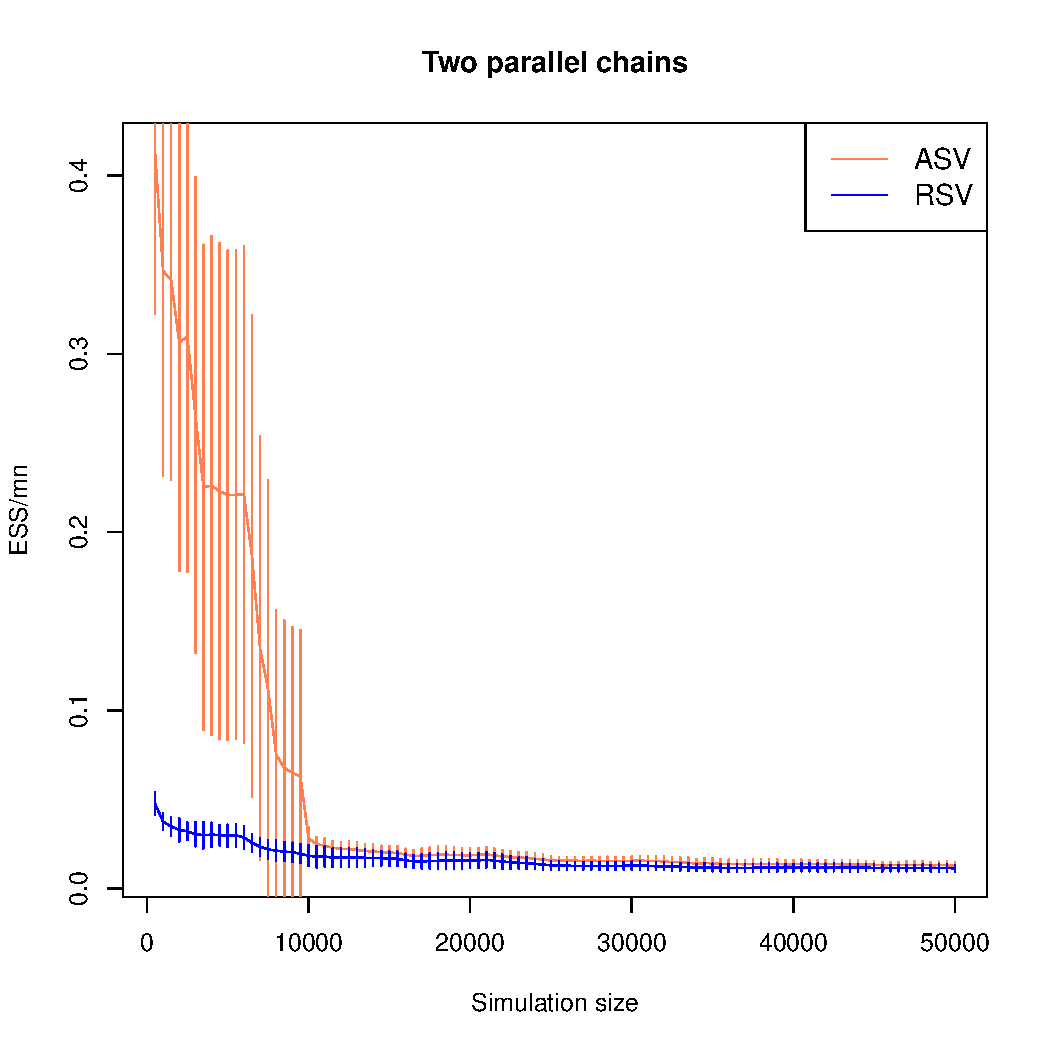
\includegraphics[width = 1.1\textwidth]{plots/boom-ess1.pdf}
      \caption{$A = 1, \; B = 3, \; C = 8$}
      \label{subfig:boom-ess1}
    \end{subfigure} \hspace{1cm}
    \begin{subfigure}[h]{.3\textwidth}
      \centering
      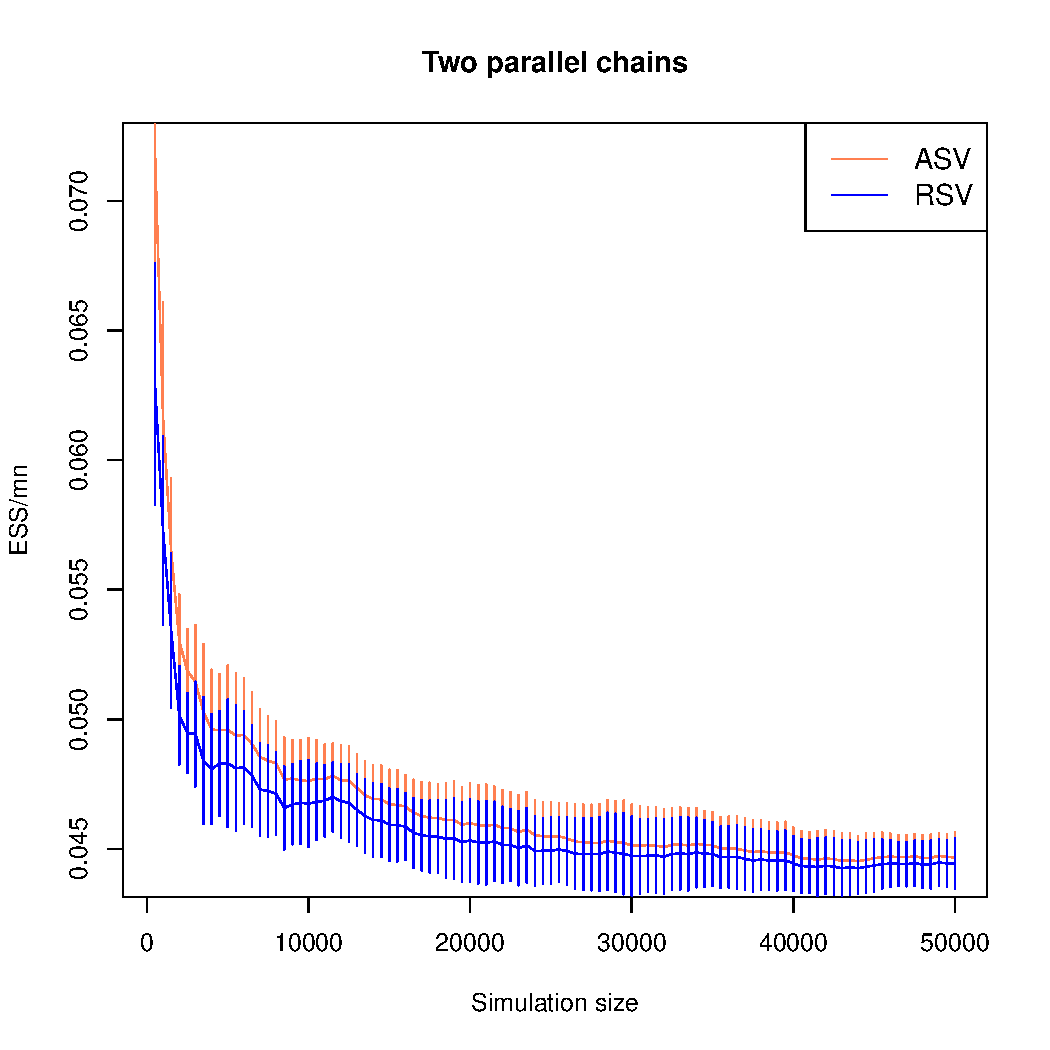
\includegraphics[width = 1.1\textwidth]{plots/boom-ess2.pdf}
      \caption{$A = 1, \; B=10, \; C = 7 $}
      \label{subfig:boom-ess2}
    \end{subfigure}
    \caption{Running plot for $\hat{\text{ESS}}/mn$ using ASV and G-SVE  for $m = 2$.}
    \label{fig:boom-ess}
\end{figure}


To examine the performance of G-SVE for a nicely mixing Markov chain, we use the parametrization of $A = 1, \; B = 10, \; C=7$. This is also a bimodal distribution, however, the two modes interact well with each other (Figure \ref{subfig:boom-pers_1_10_7}). In Figure \ref{fig:boom-ess_1_10_7}, we observe that both G-SVE and A-SVE give almost the same estimates for ESS. Similar is the case with coverage probabilities in Table \ref{table:boom-coverage_1_10_7} for a $95\%$ confidence region.

\begin{table}[htbp]
\centering
    \begin{tabular}{|c|l|l|l|l|}
    % \toprule
    \hline
        $n$ & \multicolumn{2}{|c|}{$m = 2$} & \multicolumn{2}{|c|}{$m=5$}\\
        \hline
        & ASV & G-SVE & ASV & G-SVE\\
        \hline
        $10000$ & 0.873 & 0.884 & 0.875 & 0.898   \\
        $2000$ & 0.881 &  0.888 & 0.897    & 0.914     \\
        $5000$  & 0.902 & 0.908 &  0.919 & 0.929\\
        $10000$  & 0.923 & 0.927 & 0.925 & 0.926 \\
        $50000$ & 0.951& 0.952 & 0.939 & 0.939  \\ \hline
    % \bottomrule
    \end{tabular}
    \caption{Coverage probabilities for parameter values $A = 1,\; B = 10,\; C = 7$. }
    \label{table:boom-coverage_1_10_7}
\end{table}

\subsection{Sensor Network Localization}

For our third example, we consider a real-life problem of sensor locations previously discussed by \cite{ihler2005nonparametric}. The goal is to identify unknown sensor locations using noisy distance data. This problem is specifically interesting in our case because the joint posterior distribution for missing sensor locations is multi-modal. 

\cite{tak2018repelling} modified the simulation settings of \cite{lan2014wormhole} to include only six sensor locations (four unknown and two unknown) out of eleven locations (eight known and three unknown). Following \cite{tak2018repelling}, we assume that there are six sensors scattered on a planar region where $x_i = (x_{i1}, x_{i2})^T$ denote the $2d$ coordinates of $i^{th}$ sensor. Let $y_{ij} = (y_{ji})$ denote the distance between the sensors $x_i$ and $x_j$. The distance between $x_i$ and $x_j$ is observed with probability $\pi (x_i, x_j) = \exp{\|x_i - x_j\|^2 / 2R^2}$ and with a Gaussian measurement error of $\sigma^2$. Let $z{ij}$ denote the indicator variable which is equal to 1 when the distance between $x_i$ and $x_j$ is observed. The probability model is then,
%
\begin{align*}
    z_{ij} \mid x_1, ..., x_6 &\ sim \text{Bernoulli}\left(\exp\left(\dfrac{-\|x_i - x_j\|^2}{2R^2}\right)\right)\\
    y_{ij} \mid w_{ij} = 1, x_1, ..., x_6 &\sim N(\|x_i - x_j\|^2, \sigma^2)
\end{align*}
%
\cite{ahn2013distributed} suggested the value of $R = 0.3$ and $\sigma = 0.02$. We use a Gaussian prior for the unknown locations with  mean equal to $(0,0)$ and covariance matrix equal to $100 I_2$. $y_{ij}$ is specified only if $w_{ij} = 1$. The likelihood function is then,
%
\begin{multline*}
    L(x_1, x_2, x_3, x_4) \propto \\
\prod_{j>i} \left[ \left(\exp\left(\dfrac{-\|x_i - x_j\|^2}{2 \times 0.3^2}\right)\right)^{w_{ij}} \left(1 - \exp\left(\dfrac{-\|x_i - x_j\|^2}{2 \times 0.3^2}\right)\right)^{1 - w_{ij}} \exp \left(-\dfrac{y_{ij} - \|x_i - x_j\|^2}{2 \times 0.02^2}\right)\right]    
\end{multline*}

The full posterior distribution with Gaussian prior is given by,
\begin{equation} \label{ex:sensor_post}
    \pi (x_1, x_2, x_3, x_4 | y, w) \propto 
    L(x_1, x_2, x_3, x_4) \times \exp \left(- \dfrac{\sum_{i = 1}^{4} x_i^Tx_i}{2 \times 0.02^2}\right) 
\end{equation}

where $y = (y_{ij}, j>i)$ and $w = (w_{ij}, j>i)$. We follow the Markov chain structure as described by \cite{tak2018repelling} and sample from the four bivariate conditionals for each sensor location using a Gibbs sampler. In their paper on Repelling AttG-tive Metropolis (RAM) algorithms, \cite{tak2018repelling} compare the performance of three different sampling techniques namely - Metropolis, RAM and Tempered Transitions (TT). RAM is shown to improve the acceptance rate by a factor of at least 5.5 over Metropolis using the same jumping scale. RAM algorithm supplies Markov chains with higher jumping frequency between the modes of a multimodal target distribution.\\

\begin{figure}[htbp]
    \centering
    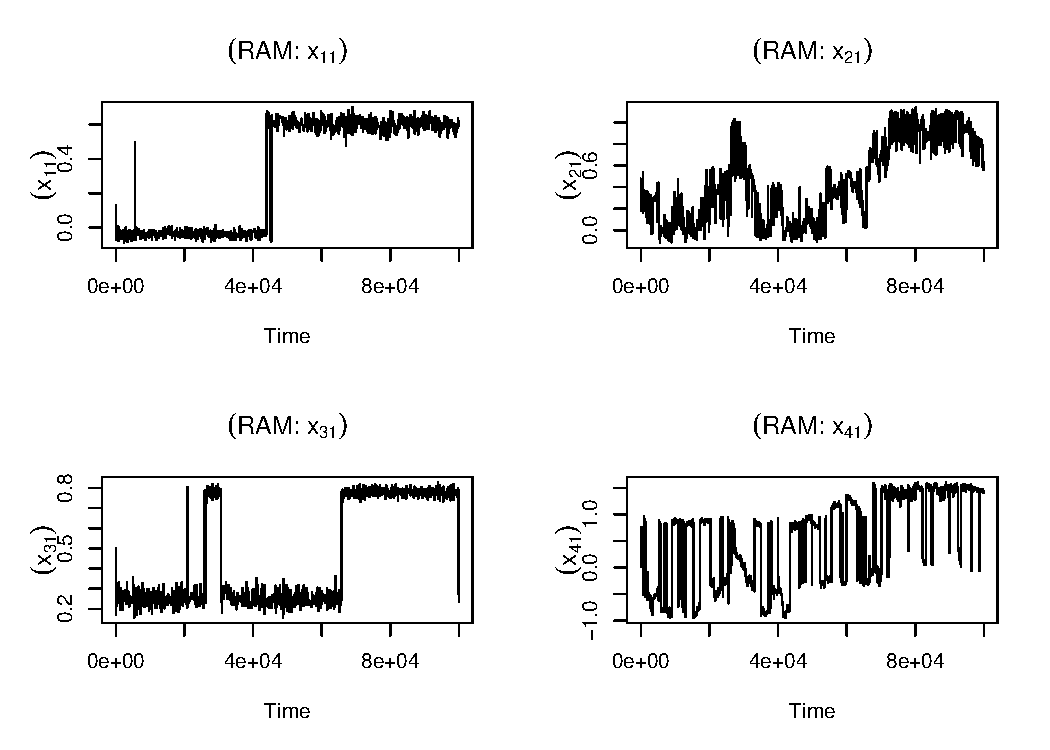
\includegraphics[width = .7\textwidth]{plots/sensor-trace.pdf}
    \caption{trace plots for the x-component of all four locations of the third chain.}
    \label{fig:sensor-trace-3}
\end{figure}

% \begin{figure}[h]
%     \centering
%     \begin{subfigure}[h]{.8\textwidth}
%       \centering
%       \includegraphics[width = \textwidth, height = 2in]{plots/sensoG-ACF-n1000.pdf}
%       \caption{$n = 10^3$}
%       \label{subfig:sensoG-ACF_n1e3}
%     \end{subfigure}
%     \begin{subfigure}[h]{.8\textwidth}
%       \centering
%       \includegraphics[width = \textwidth, height = 2in]{plots/sensoG-ACF-n1e5.pdf}
%       \caption{$n = 10^5$}
%       \label{subfig:sensoG-ACF_n1e5}
%     \end{subfigure}
%     \caption{ACF and G-ACF for component-3 of chain-3 at two different number of Monte Carlo samples. }
%     \label{fig:sensoG-ACF}
% \end{figure}


We will use the RAM algorithm with a jumping scale equal to $0.5$ to sample five parallel Markov chains with well-separated starting points. The total simulation size for each chain is fixed at $100,000$. Figure \ref{fig:sensor-trace-3} demonstrates the trace plots of the first chain for the x-component of all four unknown locations. We observe the bi-modal nature of the marginal distribution for each component. The Markov chains get stuck at a particular mode for a long time before jumping to the other mode. Figure \ref{fig:sensoG-ACF} shows the effect of this "sticky" nature of Markov chains over the autocorrelations centered around the local and global mean. For a small sample size of 1000, it can be seen that the third chain has not explored the sample space well. As a consequence, the local mean differs a lot from the global mean (averaged over all five chains).

 
\section{Discussion} \label{sec:discussion}
 

\appendix

\section{Appendix}  \label{sec:appendix}
\subsection{Preliminaries} \label{apdx:preliminaries}

\begin{lemma}
\label{lemma: brownian}
(\cite{csorgo2014strong}). Suppose Assumption \ref{ass:sip} holds, then for all $\epsilon > 0$ and for almost all sample paths, there exists $n_{0}\left(\epsilon\right)$ such that $\forall n\geq n_{0}$ and $\forall i = 1, ..., p$

\[
\sup_{0\leq t \leq n-b_n}\sup_{0 \leq s \leq b_n} \left| B^{\left(i\right)}\left(t+s\right) - B^{\left(i\right)}\left(t\right) \right| < \left(1+ \epsilon\right)\left(2b_n\left(\log\dfrac{n}{b_n} + \log\; \log\; n\right)\right)^{1/2} ,
\]
%
\[
\sup_{0 \leq s \leq b_n} \left|B^{\left(i\right)}\left(n\right) - B^{\left(i\right)}\left(n - s\right)\right| < \left(1+ \epsilon\right)\left(2b_n\left(\log\dfrac{n}{b_n} + \log\;\log\;n\right)\right)^{1/2} , \;and
\]
%
\[
\left|B^{\left(i\right)}\left(n\right)\right| < \left(1+\epsilon\right)\sqrt{2n\;\log \log n} \; . 
\]
\end{lemma}


% \begin{lemma} \label{lemma:consis_1}
%   If Assumption~\ref{ass:sip} holds, then $\| \bar{\bar{X}} - \mu\|_{\infty}, \|\bar{X}_s - \mu\|_{\infty} \xrightarrow[]{a.s.} 0$ as $n \to \infty$ for all $s \in \{1,..., m\}$\\
%   \end{lemma}

% \begin{proof}
% Let $\|.\|$ denote the Euclidean norm. Assumption \ref{ass:sip} allows us to upper bound $\|\bar{X}_s - \mu\|_{\infty}$ using SIP. Following that, we show that the upper bound term converges to 0 as $n \to \infty$ using lemma \ref{lemma: brownian}.
%  \begin{align*}
%     \|\bar{X}_s - \mu\|_{\infty} & \leq \|\bar{X}_s - \mu\| \\
%     &= \dfrac{1}{n}\left\|\sum_{t=1}^{n}X_{st} - n\mu\right\| = \dfrac{1}{n}  \left \|\sum_{t=1}^{n}X_{st} - n\mu \pm L B(n) \right\|\\
%     & \leq \dfrac{1}{n}\left\|\sum_{t=1}^{n}X_{st} - \mu - L B(n)\right\| + \dfrac{\left\|L B(n)\right\|}{n}\\
%     &< \dfrac{D\psi(n)}{n} + \dfrac{\|L B(n)\|}{n}\\
%     &< \dfrac{D\psi(n)}{n} + \dfrac{1}{n}\|L\| \left(\sum\limits_{i=1}^{p}|B^{(i)}(k)|^2\right)^{1/2}\\
%     & \leq \dfrac{D\psi(n)}{n} + \dfrac{1}{n}\|L\| p^{1/2}(1+\epsilon)\sqrt{2n \log\log n}\\
%     & \xrightarrow[]{a.s.} 0\;\; as \;\; n\to \infty
%  \end{align*}
% %
% Similarly one can easily show that $\|\bar{\bar{X}} - \mu\|_{\infty} \to 0$ as $n \to \infty$ using the same upper-bound as:
% % 
% \begin{align*}
%     \|\bar{\bar{X}} - \mu\|_{\infty} & \leq \|\bar{\bar{X}} - \mu\| = \dfrac{1}{m}\left \|\sum_{j=1}^{m}(\bar{X}_j- \mu) \right\| \leq \dfrac{1}{m}\sum_{j=1}^{m}\|\bar{X}_j - \mu\| \xrightarrow{a.s.} 0 \, \textrm{as } n \to \infty 
% \end{align*}
% \end{proof}


% \section{Proof of Theorems} \label{appendix:A}

\subsection{Proof of Theorem~\ref{th:G-_expec}} 
\label{appendix:bias}

 % \begin{proof}[Proof of Theorem~\ref{th:G-_expec}]
% \begin{lemma} \label{lemma:bias1}
% $\mathbb{E}\left[ \left(X_{11} - \bar{X}_1 \right) \left(\bar{X}_1 - \bar{\bar{X}} \right)^T \right] = \dfrac{m-1}{mn}\left(\sum\limits_{k=0}^{n-1}\Gamma(k) - \Sigma\right)$
% \end{lemma}
% \begin{proof}
% \begin{align*}
%     &\mathbb{E} \left[ \left(X_{11} - \bar{X}_1 \right) \left(\bar{X}_1 - \bar{\bar{X}} \right)^T \right]\\
%      &= \mathbb{E} \left[X_{11}\bar{X}_1^T \right] - \mathbb{E}\left[X_{11}\bar{\bar{X}}^T \right] + \mathbb{E} \left[\bar{X}_1\bar{\bar{X}}^T \right] - \mathbb{E} \left[\bar{X}_1\bar{X}_1^T \right]\\
%     &= \mathbb{E} \left[X_{11}\bar{X}_1^T \right] - \dfrac{1}{m}\mathbb{E} \left[X_{11}\bar{X}_1^T \right] - \dfrac{m-1}{m}\mathbb{E} \left[X_{11}\bar{X}_2^T \right] + \dfrac{1}{m}\mathbb{E} \left[\bar{X}_1\bar{X}_1^T \right] + \dfrac{m-1}{m}\mathbb{E} \left[\bar{X}_1\bar{X}_2^T \right] - \mathbb{E} \left[\bar{X}_1\bar{X}_1^T \right]\\
%     &= \dfrac{m-1}{m}\left(\mathbb{E} \left[X_{11}\bar{X}_1^T \right] - \mathbb{E} \left[X_{11}\bar{X}_2^T \right] + \mathbb{E} \left[\bar{X}_1\bar{X}_2^T \right] - \mathbb{E} \left[\bar{X}_1\bar{X}_1^T \right]\right)\\
%     &= \dfrac{m-1}{m}\left(\dfrac{1}{n}\sum_{t=1}^{n}\mathbb{E} \left[X_{11}X_{1t}^T \right] - \mathbb{E}\left[X_{11}\right] \mathbb{E}\left[\bar{X}_2^T \right] + \mathbb{E} \left[\bar{X}_1\right]\mathbb{E}\left[\bar{X}_2^T\right] - \text{Var}\left[\bar{X}_1 \right] - \mathbb{E}\left[\bar{X}_1 \right]\mathbb{E}\left[\bar{X}_1^T \right]\right)\\
%     &= \dfrac{m-1}{m}\left(\dfrac{1}{n}\sum_{k=0}^{n-1}\Gamma(k) + \mu \mu^T - \mu \mu^T + \mu \mu^T - \text{Var}\left[\bar{X}_1 \right] - \mu \mu^T\right)\\
%     &= \dfrac{m-1}{mn}\left(\sum_{k=0}^{n-1}\Gamma(k) - n\text{Var}\left[\bar{X}_1 \right]\right)\,.
% \end{align*}
% %
% Similarly,
% %    
% \begin{align*}
%     \mathbb{E} \left[ \left(\bar{X}_1 - \bar{\bar{X}} \right)  \left(X_{11} - \bar{X}_1 \right)^T \right] &= \mathbb{E}\left[ \left(X_{11} - \bar{X}_1 \right) \left(\bar{X}_1 - \bar{\bar{X}} \right)^T \right]^T = \dfrac{m-1}{mn}\left(\sum_{k=0}^{n-1}\Gamma(k) - \Sigma \right)^T\,.
%     % &= \dfrac{m-1}{mn}\left(\sum_{k=0}^{n-1}\Gamma(k) - \Sigma \right)\\
% \end{align*}
% \end{proof}


% \begin{lemma} \label{lemma:bias2}
% \[
% \mathbb{E}\left[\sum\limits_{s=1}^{m} \left(\bar{X}_{s} - \bar{\bar{X}} \right) \left(\bar{X}_{s} - \bar{\bar{X}} \right)^{T}\right] =  (m-1)\text{Var}(\bar{X}_1)\,.
% \]
% \end{lemma}

% % $\bar{X}_i$ are independently and identically distributed for all $i$; this implies $\Var(\bar{\bar{X}}) = \dfrac{1}{m} \Var(\bar{X}_1)$. 

% \begin{proof}
% \begin{align*}
% \mathbb{E}\left[\sum_{s=1}^{m} \left(\bar{X}_{s} - \bar{\bar{X}} \right)  \left(\bar{X}_{s} - \bar{\bar{X}} \right)^{T}\right] &= \mathbb{E}\left[\sum_{s=1}^{m}\bar{X}_{s}\bar{X}_{s}^{T} -\sum_{s=1}^{m}\bar{X}_{s}\bar{\bar{X}}^{T} - \bar{\bar{X}}^{T}\sum_{s=1}^{m}\bar{X}_{s}^{T} + m\bar{\bar{X}}\bar{\bar{X}}^{T}\right]\\
% &= \mathbb{E}\left[\sum_{s=1}^{m}\bar{X}_{s}\bar{X}_{s}^{T} - m\bar{\bar{X}}\bar{\bar{X}}^{T}\right]\\
% &= m\left(\mathbb{E}\left[\bar{X}_{1}\bar{X}_{1}^{T}\right] - \mathbb{E}\left[\bar{\bar{X}}\bar{\bar{X}}^{T}\right]\right)\\
% &= m\left(\Var(\bar{X}_{1}) + \mu\mu^{T} - \Var(\bar{\bar{X}}) - \mu\mu^{T}\right)\\
% &= (m-1)\Var(\overline{X_1})\,.
% \end{align*}
% \end{proof}



\begin{align*}
\hat{\Gamma}_{G,s}(k) & = \dfrac{1}{n}\sum_{t=1}^{n-|k|} \left(X_{st} - \bar{\bar{X}} \right) \left(X_{s(t+k)} - \bar{\bar{X}} \right)^T \\
    &= \left[\dfrac{1}{n} \sum_{t=1}^{n-|k|} \left(X_{st} - \bar{X}_s \right) \left(X_{s(t+k)} - \bar{X}_s \right)^T \right] + \left[\dfrac{1}{n} \sum_{t=1}^{|k|} \left(\bar{X}_s - \bar{\bar{X}} \right)  \left(\bar{X}_s - X_{st} \right)^T\right] \\ 
    & \quad +  \left[\dfrac{1}{n} \sum_{t=n-|k|+1}^{n}  \left( \bar{X}_s - X_{st} \right)  \left(\bar{X}_s - \bar{\bar{X}} \right)^T\right] + \left[\dfrac{n-|k|}{n} \left(\bar{X}_s - \bar{\bar{X}}\right)   \left(\bar{X}_s - \bar{\bar{X}} \right)^T\right]\\
    &= \hat{\Gamma}_s(k) - \dfrac{1}{n} \sum_{t=1}^{|k|}A_{st}^T - \dfrac{1}{n}\sum_{t=n-|k|+1}^{n}A_{st} + \dfrac{n-|k|}{n}  \left(\bar{X}_s - \bar{\bar{X}} \right)  \left(\bar{X}_s - \bar{\bar{X}} \right)^T\,, \numberthis \label{eq:acf_breakdown}
\end{align*}
%
where $A_{st} = (X_{st}-\bar{X}_s)(\bar{X}_s - \bar{\bar{X}})^T$. We will study the expectations of the each of the above terms. Without loss of generality, consider $A_{11}$,
\begin{align*}
    &\E \left[A_{11} \right]\\
     &= \mathbb{E} \left[ \left(X_{11} - \bar{X}_1 \right) \left(\bar{X}_1 - \bar{\bar{X}} \right)^T \right]\\
     % &= \mathbb{E} \left[X_{11}\bar{X}_1^T \right] - \mathbb{E}\left[X_{11}\bar{\bar{X}}^T \right] + \mathbb{E} \left[\bar{X}_1\bar{\bar{X}}^T \right] - \mathbb{E} \left[\bar{X}_1\bar{X}_1^T \right]\\
    &= \mathbb{E} \left[X_{11}\bar{X}_1^T \right] - \dfrac{1}{m}\mathbb{E} \left[X_{11}\bar{X}_1^T \right] - \dfrac{m-1}{m}\mathbb{E} \left[X_{11}\bar{X}_2^T \right] + \dfrac{1}{m}\mathbb{E} \left[\bar{X}_1\bar{X}_1^T \right] + \dfrac{m-1}{m}\mathbb{E} \left[\bar{X}_1\bar{X}_2^T \right] - \mathbb{E} \left[\bar{X}_1\bar{X}_1^T \right]\\
    &= \dfrac{m-1}{m}\left(\mathbb{E} \left[X_{11}\bar{X}_1^T \right] - \mathbb{E} \left[X_{11}\bar{X}_2^T \right] + \mathbb{E} \left[\bar{X}_1\bar{X}_2^T \right] - \mathbb{E} \left[\bar{X}_1\bar{X}_1^T \right]\right)\\
    &= \dfrac{m-1}{m}\left(\dfrac{1}{n}\sum_{t=1}^{n}\mathbb{E} \left[X_{11}X_{1t}^T \right] - \mathbb{E}\left[X_{11}\right] \mathbb{E}\left[\bar{X}_2^T \right] + \mathbb{E} \left[\bar{X}_1\right]\mathbb{E}\left[\bar{X}_2^T\right] - \text{Var}\left[\bar{X}_1 \right] - \mathbb{E}\left[\bar{X}_1 \right]\mathbb{E}\left[\bar{X}_1^T \right]\right)\\
    % &= \dfrac{m-1}{m}\left(\dfrac{1}{n}\sum_{k=0}^{n-1}\Gamma(k) + \mu \mu^T - \mu \mu^T + \mu \mu^T - \text{Var}\left[\bar{X}_1 \right] - \mu \mu^T\right)\\
    &= \dfrac{m-1}{mn}\left(\sum_{k=0}^{n-1}\Gamma(k) - n\text{Var}\left[\bar{X}_1 \right]\right)\,. \numberthis \label{eq:acf_2}
\end{align*}
%
Similarly,
%    
\begin{align}
\label{eq:acf_3}
    \mathbb{E} \left[ A_{11}^T \right] &= \mathbb{E}\left[ A_{11}\right]^T = \dfrac{m-1}{mn}\left(\sum_{k=0}^{n-1}\Gamma(k)^T - n\text{Var}\left[\bar{X}_1 \right] \right)\,.
    % &= \dfrac{m-1}{mn}\left(\sum_{k=0}^{n-1}\Gamma(k) - \Sigma \right)\\
\end{align}


Further,
\begin{align*}
\mathbb{E}\left[ \left(\bar{X}_{1} - \bar{\bar{X}} \right)  \left(\bar{X}_{1} - \bar{\bar{X}} \right)^{T}\right] &= \mathbb{E}\left[ \bar{X}_{1}\bar{X}_{1}^{T} - \bar{X}_{1}\bar{\bar{X}}^{T} - \bar{\bar{X}} \bar{X}_{1}^{T} + \bar{\bar{X}}\bar{\bar{X}}^{T}\right]\\
% &= \mathbb{E}\left[ \bar{X}_{1}\bar{X}_{1}^{T} - \bar{\bar{X}}\bar{\bar{X}}^{T}\right]\\
% &= \left(\mathbb{E}\left[\bar{X}_{1}\bar{X}_{1}^{T}\right] - \mathbb{E}\left[\bar{\bar{X}}\bar{\bar{X}}^{T}\right]\right)\\
&= \left(\Var(\bar{X}_{1}) + \mu\mu^{T} - \Var(\bar{\bar{X}}) - \mu\mu^{T}\right)\\
&= \dfrac{m-1}{m}\Var(\bar{X}_1)\,. \numberthis \label{eq:acf_4}
\end{align*}
%
Additionally, the locally-centered autocovariance exhibits the following expectation
 \begin{equation} \label{eq:priestly}
     \mathbb{E}[\hat{\Gamma}(k)] = \left(1- \dfrac{\abs{k}}{n}\right)\left(\Gamma(k) - \Var{(\bar{X})}
 \right)\,.
 \end{equation}
%
Using \eqref{eq:priestly}, \eqref{eq:acf_2}, \eqref{eq:acf_3}, and \eqref{eq:acf_4} in \eqref{eq:acf_breakdown},
\begin{align*}
    & \E \left[\hat{\Gamma}_{G,s}(k) \right] \\
    &= \mathbb{E}\left[\hat{\Gamma}_{s}(k)\right] - \dfrac{1}{n} \left(\sum\limits_{t=1}^{|k|}\mathbb{E}[A_{1t}^T] + \sum\limits_{t=n-|k|+1}^{n}\mathbb{E}[A_{1t}]\right) + \left(1- \dfrac{|k|}{n}\right)\left(1-\dfrac{1}{m}\right)\Var(\bar{X}_1)\\
    &= \mathbb{E}\left[\hat{\Gamma}_{s}(k)\right] - \dfrac{|k|}{n}\left(1-\dfrac{1}{m}\right)\left(\dfrac{1}{n}\sum_{h=0}^{n-1}\Gamma(h) + \dfrac{1}{n}\sum_{h=0}^{n-1}\Gamma(h)^T - 2 \Var(\bar{X}_1)\right) + \left(1- \dfrac{|k|}{n}\right)\left(1-\dfrac{1}{m}\right)\Var(\bar{X}_1)\\
    &= \left(1- \dfrac{|k|}{n}\right)\Gamma(k) - \dfrac{|k|}{n}\left[\left(1-\dfrac{1}{m}\right)\left(\dfrac{1}{n}\sum_{h=0}^{n-1}\Gamma(h)^T + \dfrac{1}{n}\sum_{h=0}^{n-1}\Gamma(h)\right) - \left(2-\dfrac{1}{m}\right) \Var(\bar{X}_1)\right] - \dfrac{\Var(\overline{X}_1)}{m}\,.
\end{align*}
%
 We can use the results of \cite{song1995optimal} given in \eqref{eq:song} to expand $\Var(\bar{X}_1)$. Expectation of $\hat{\Gamma}_{G,s}(k)$ can then broken down as following,
 \begin{equation} \label{eq:G-_expec_breakdown}
     \mathbb{E}\left[\hat{\Gamma}_{G,s}(k)\right] = \left(1- \dfrac{|k|}{n}\right)\Gamma(k) + O_1 + O_2\,.
 \end{equation}
%
where,
\begin{align*}
    O_1 &= -\dfrac{|k|}{n}\left[\left(1-\dfrac{1}{m}\right)\left(\dfrac{1}{n}\sum_{h=0}^{n-1}\Gamma(h)^T + \dfrac{1}{n}\sum_{h=0}^{n-1}\Gamma(h)\right) - \left(2-\dfrac{1}{m}\right) \left(\dfrac{\Sigma}{n} + \dfrac{\Phi}{n^2}\right)\right] \, ,\\
    O_2 &= -\dfrac{1}{m}\left(\dfrac{\Sigma}{n} + \dfrac{\Phi}{n^2}\right) + o(n^{-2})
\end{align*}
%
We observe that both $O_1 \textrm{ and } O_2$ are small order terms that converge to 0 as $n \to \infty$. Here, $O_1 = (-\abs{k}/n)\mathcal{O}(1/n) \textrm{ and } O_2 = {\color{red}\mathcal{O}}(1/n)$. For a diagonal element of $\Gamma$,
% We observe that this expectation result is very similar to equation \ref{eq:priestly} from \cite{priestley1981spectral} for the asymptotically unbiased estimator of autocovariance except for an additional positive bias term. This helps in countering the inherent negative bias in $\hat{\Gamma}(k)$ and give more informative estimates of autocovariance.  Although, bias term for a fixed $k$ is $o(1)$, it increases with $k$. We have explicitly written the end effect term arising from using the estimator $\bar{\bar{X}}$ for $\mu$. These are small order terms that vanish as $n \to \infty$.
%
\begin{align*}
& \E \left[ \hat{\Gamma}_{G,s}^{ii}\right]\\
& = \mathbb{E}\left[\hat{\Gamma}^{ii}_{s}(k)\right] - \dfrac{|k|}{n}\left[\left(1-\dfrac{1}{m}\right)\left(\dfrac{1}{n}\sum_{h=0}^{n-1} \left[\Gamma^{ii}(h)^T + \Gamma^{ii}(h) \right] \right) - \left(2-\dfrac{1}{m}\right) \Var(\overline{X}_1)^{ii}\right] - \dfrac{\Var(\overline{X}_1)^{ii}}{m}\,.
\end{align*}
In the presence of positive correlation, the leftover term is positive.


% \begin{proof}[Proof of corollary \ref{cor:lag0_expectation}]

% \begin{align*}
%     \hat{\Gamma}_{G-}(0) &= \dfrac{1}{m}\sum_{s=1}^{m}\hat{\Gamma}_{G-,s}(0) = \dfrac{1}{mn}\sum_{s=1}^{m}\sum_{t=1}^{n}  \left(X_{st} - \bar{\bar{X}}\right)  \left(X_{st} - \bar{\bar{X}}\right)^T\\
%     &= \left[\dfrac{1}{mn}\sum_{s=1}^{m}\sum_{t=1}^{n} \left(X_{st} - \bar{X}_s \right)  \left(X_{st} - \bar{X}_s \right)^T\right] + \left[\dfrac{1}{m}\sum_{s=1}^{m} \left(\bar{X}_s - \bar{\bar{X}} \right) \left(\bar{X}_s - \bar{\bar{X}} \right)^T\right]\\
%     &= \dfrac{1}{m}\sum_{s=1}^{m}\hat{\Gamma}_s(0)  + \dfrac{1}{m}\sum_{s=1}^{m} \left(\bar{X}_s - \bar{\bar{X}} \right)  \left(\bar{X}_s - \bar{\bar{X}} \right)^T\,.
% \end{align*}
% Using \eqref{eq:priestly} and \eqref{eq:acf_4} the expectation of $\hat{\Gamma}_{G-}(0)$ can be written as 
% %
% \begin{align*}
%     \mathbb{E} \left[\hat{\Gamma}_{G-}(0) \right] &= \E\left[\hat{\Gamma}_1(0) \right] + \left(1-\dfrac{1}{m}\right)\Var(\bar{X}_1) \\
%     & = \Gamma(k) - \dfrac{1}{m}\Var(\bar{X}_1)\,.
%     % &= \Gamma(0) - \dfrac{\Sigma}{mn} - \dfrac{\Phi}{mn^2} + o(n^{-2})
% \end{align*}

% \end{proof}


\subsection{Strong consistency argument} \label{appendix:strong_consis}


Consider pseudo spectral variance estimators for the $s$th chain, denoted by $\tilde{\Sigma}_s$ which uses data centered around the unobserved actual mean $\mu$:
\begin{align*}
    \tilde{\Gamma}_s(k) &= \dfrac{1}{n}\sum_{t=1}^{n-|k|}(X_{st}-\mu)(X_{s(t+k)}-\mu)^T \\ 
    \tilde{\Sigma}_s &= \sum_{k=-b_n+1}^{b_n-1}w\left(\dfrac{k}{b_n}\right)\tilde{\Gamma}_s(k) \,.
\end{align*}
%
The average pseudo spectral variance estimator is
\[
\tilde{\Sigma} = \dfrac{1}{m}\sum\limits_{s=1}^{m}\tilde{\Sigma}_s
\]

Further, let
\begin{align*}
  M_1 & = \dfrac{1}{m}\sum\limits_{s=1}^{m}\left\{\sum\limits_{k=-b_n+1}^{b_n-1}w\left(\dfrac{k}{b_n}\right)\sum\limits_{t=1}^{n-|k|}\dfrac{1}{n}\left[ \left(X_{st}-\mu \right)_i   \left(\mu-\bar{\bar{X}} \right)_j +    \left(\mu-\bar{\bar{X}} \right)_i  \left(X_{s(t+k)}-\mu \right)_j \right]\right\}\,, \\ 
  %
M_2 &= \left(\mu-\bar{\bar{X}} \right)_i   \left(\mu-\bar{\bar{X}} \right)_j\sum\limits_{k=-b_n+1}^{b_n-1}\left(1-\dfrac{|k|}{n}\right)w\left(\dfrac{k}{b_n}\right)\,.
\end{align*}


\begin{lemma} \label{lemma:G-SVE_breakdown}
For the G-SVE estimator, $\hat{\Sigma}_{G}^{ij} = \tilde{\Sigma}^{ij} + M_1 + M_2$ and 
\[
|M_1 + M_2| \leq D^2 g_1(n) + D g_2(n) + g_3(n)\,,
\]
where
\begin{align*}
    g_1(n) &= (4+C_1)\dfrac{b_n \psi^2(n)}{n^2} - 4\dfrac{\psi^2(n)}{n^2} \to 0\\
    g_2(n) &= 2\sqrt{2}\|L\|p^{1/2}(1+\epsilon)\left[(4+C_1)\dfrac{b_n\psi(n)\sqrt{n\log \log n}}{n^2} - 4\dfrac{\psi(n)\sqrt{n\log \log n}}{n^2}\right] \to 0\\
    g_3(n) &= \|L\|^2 p (1+\epsilon)^2\left[(4+C_1)\dfrac{b_n \log\log n}{n} - 4 \dfrac{\log \log n}{n}\right] \to 0\,.
\end{align*}
\end{lemma}

\begin{proof}
The proof follows from standard algebraic calculations and is presented here for completeness. Consider,
\begin{align*}
\hat{\Sigma}_{G}^{ij} &= \dfrac{1}{m}\sum_{s=1}^{m} \sum_{k=-b_n+1}^{b_n-1}w\left(\dfrac{k}{b_n}\right)\dfrac{1}{n}\sum_{t=1}^{n-|k|} \left(X_{st}-\bar{\bar{X}} \right)_i \left(X_{s(t+k)}-\bar{\bar{X}} \right)_j\\
% &= \dfrac{1}{m}\sum_{s=1}^{m}\sum_{k=-b_n+1}^{b_n-1}w\left(\dfrac{k}{b_n}\right)\dfrac{1}{n}\sum_{t=1}^{n-|k|} \left[  \left\{\left(X_{st}-\mu \right)_i + \left(\mu-\bar{\bar{X}} \right)_i \right \}  \left\{ \left(X_{s(t+k)}-\mu \right)_j + \left(\mu-\bar{\bar{X}} \right)_j \right \} \right]\\
&= \dfrac{1}{m}\sum_{s=1}^{m}\sum_{k=-b_n+1}^{b_n-1}w\left(\dfrac{k}{b_n}\right)\dfrac{1}{n}\sum_{t=1}^{n-|k|}  \left[ \left(X_{st}-\mu \right)_i  \left(X_{s(t+k)}-\mu \right)_j+  \left(X_{st} - \mu \right)_i    \left(\mu - \bar{\bar{X}} \right)_j \right. \\  
& \quad + \left. \left(\mu-\bar{\bar{X}} \right)_i  \left(X_{s(t+k)}-\mu \right)_j + \left(\mu-\bar{\bar{X}} \right)_i  \left(\mu-\bar{\bar{X}}  \right)_j  \right]\\
& = \tilde{\Sigma}^{ij} + \left[(\mu-\bar{\bar{X}})_i(\mu-\bar{\bar{X}})_j\sum_{k=-b_n+1}^{b_n-1}\left(1-\dfrac{|k|}{n}\right)w\left(\dfrac{k}{b_n}\right)\right] \\ 
& \quad  + \dfrac{1}{m}\sum_{s=1}^{m}\sum_{k=-b_n+1}^{b_n-1}  w\left(\dfrac{k}{b_n}\right)\sum_{t=1}^{n-|k|}  \left[\dfrac{1}{n} \left(X_{st} - \mu \right)_i \left(\mu - \bar{\bar{X}} \right)_j + \dfrac{1}{n} \left(\mu-\bar{\bar{X}} \right)_i  \left(X_{s(t+k)}-\mu \right)_j \right] \\ 
& = \tilde{\Sigma}^{ij} + M_1 + M_2\,.
\end{align*}

Consequently
\[
\left|\hat{\Sigma}_{G}^{ij} - \tilde{\Sigma}^{ij}  \right| = |M_1 + M_2| \leq |M_1| + |M_2|\,.
\]
%
We first present a result which will be useful to use later. For any Markov chain $s$, 
\begin{align*}
  \|\bar{X}_s - \mu\|_{\infty} & \leq \|\bar{X}_s - \mu\| = \dfrac{1}{mn}\left\|\sum_{t=1}^{n}X_{st} - n\mu\right\| \\
  % &= \dfrac{1}{n}  \left \|\sum_{t=1}^{n}X_{st} - n\mu \pm L B(n) \right\|\\
  & \leq \dfrac{1}{n}\left\|\sum_{t=1}^{n}X_{st} - n \mu - L B(n)\right\| + \dfrac{\left\|L B(n)\right\|}{n}\\
  &< \dfrac{D\psi(n)}{n} + \dfrac{\|L B(n)\|}{n}\\
  &< \dfrac{D\psi(n)}{n} + \dfrac{1}{n}\|L\| \left(\sum\limits_{i=1}^{p}|B^{(i)}(n)|^2\right)^{1/2}\\
  & \leq \dfrac{D\psi(n)}{n} + \dfrac{1}{n}\|L\| p^{1/2}(1+\epsilon)\sqrt{2n \log\log n}\,. \numberthis \label{eq:xbars_bound}
  % & \xrightarrow[]{a.s.} 0\;\; as \;\; n\to \infty 
\end{align*}
 %
 Similarly,
 \begin{equation}
\label{eq:xbarbar_bound}
   \| \bar{\bar{X}} - \mu\|_{\infty} \leq \dfrac{D\psi(n)}{n} + \dfrac{1}{n}\|L\| p^{1/2}(1+\epsilon)\sqrt{2n \log\log n}\,.
\end{equation}
%  \begin{align*}
%   \| \bar{\bar{X}} - \mu\|_{\infty} & \leq \|\bar{\bar{X}} - \mu\| = \dfrac{1}{n}\left\|\sum_{s=1}^{m} \left(\sum_{t=1}^{n}X_{st} - n\mu \right)\right\| \\
%   &\leq \dfrac{1}{m}\sum_{s=1}^{m}\dfrac{1}{n}  \left \| \sum_{t=1}^{n}X_{st} - n\mu \pm L B(n) \right\|\\
%   & \leq \dfrac{1}{m} \sum_{s=1}^{m} \dfrac{1}{n}\left\| \sum_{t=1}^{n}X_{st} - n \mu - L B(n)\right\| + \dfrac{\left\|L B(n)\right\|}{n}\\
%   &< \dfrac{D\psi(n)}{n} + \dfrac{\|L B(n)\|}{n}\\
%   &< \dfrac{D\psi(n)}{n} + \dfrac{1}{n}\|L\| \left(\sum\limits_{i=1}^{p}|B^{(i)}(k)|^2\right)^{1/2}\\
%   & \leq \dfrac{D\psi(n)}{n} + \dfrac{1}{n}\|L\| p^{1/2}(1+\epsilon)\sqrt{2n \log\log n}\,. \numberthis \label{eq:xbarbar_bound}
%   % & \xrightarrow[]{a.s.} 0\;\; as \;\; n\to \infty 
% \end{align*}
%
Now consider,
\begin{align*}
& |M_1| \\ 
   % & = \left|\dfrac{1}{m}\sum _{s=1}^{m}\left\{\sum_{k=-b_n+1}^{b_n-1}w\left(\dfrac{k}{b_n}\right)\sum_{t=1}^{n-|k|} \dfrac{1}{n}\left[ \left(X_{st} - \mu \right)_i  \left(\mu-\bar{\bar{X}} \right)_j + \left(\mu-\bar{\bar{X}} \right)_i  \left(X_{s(t+k)} - \mu \right)_j\right]\right\}\right| \\
   % & \leq \dfrac{1}{m}\sum_{s=1}^{m}\left\{\sum_{k=-b_n+1}^{b_n-1}w\left(\dfrac{k}{b_n}\right)\left[ \dfrac{1}{n}{\left|\sum\limits_{t=1}^{n-|k|} \left(X_{st} - \mu \right)_i  \left(\mu - \bar{\bar{X}} \right)_j\right|} + \dfrac{1}{n}{\left|\sum_{t=1}^{n-|k|} \left(\mu-\bar{\bar{X}} \right)_i\left(X_{s(t+k)} - \mu \right)_j\right|} \right]\right\}\\
    & \leq \dfrac{1}{m}\sum_{s=1}^{m}\left\{\sum_{k=-b_n+1}^{b_n-1}w\left(\dfrac{k}{b_n}\right)\left[ \dfrac{1}{n}\left|\sum_{t=1}^{n-|k|}(X_{st}- \mu)_i\right|\left|(\mu-\bar{\bar{X}})_j\right|+ \dfrac{1}{n}\left|(\mu-\bar{\bar{X}})_i\right|\left|\sum_{t=1}^{n-|k|}(X_{j(t+k)}-\mu)_j\right|\right]\right\}\\
    & \leq \dfrac{\|(\bar{\bar{X}} - \mu)\|_{\infty}}{m} \sum_{s=1}^{m}\sum\limits_{k=-b_n+1}^{b_n-1}\left[ \dfrac{1}{n}\left\|\sum_{t=1}^{n-|k|}(X_{st}-\mu)\right\|_{\infty} + \dfrac{1}{n}\left\|\sum_{t=1}^{n-|k|}(X_{s(t+k)}-\mu)\right\|_{\infty} \right]\\
    &\leq \dfrac{\|(\bar{\bar{X}} - \mu)\|_{\infty}}{m} \\
    & \quad \times \sum_{s=1}^{m}\sum_{k=-b_n+1}^{b_n-1}\left[ \dfrac{1}{n}\left\|\sum_{t=n-|k|+1}^{n}(X_{st} - \mu) - n(\bar{X}_s - \mu) \right\|_{\infty} + \dfrac{1}{n}\left\|\sum_{t=1}^{|k|}(X_{st} - \mu) - n(\bar{X}_s - \mu)\right\|_{\infty} \right]\\
    &\leq \dfrac{\|(\bar{\bar{X}} - \mu)\|_{\infty}}{m} \sum_{s=1}^{m}\sum\limits_{k=-b_n+1}^{b_n-1}\left[ \dfrac{1}{n}\left\|\sum_{t=n-|k|+1}^{n}(X_{st} - \mu)\right\|_{\infty} + \dfrac{1}{n}\left\|\sum_{t=1}^{|k|}(X_{st} - \mu)\right\|_{\infty} + 2\|\bar{X}_s - \mu\|_{\infty} \right]\\
    & \leq \dfrac{\|(\bar{\bar{X}} - \mu)\|_{\infty}}{m} \sum\limits_{s=1}^{m}\sum_{k=-b_n + 1}^{b_n-1}   \dfrac{1}{n}\left[\left\|\sum_{t=n-|k|+1}^{n}(X_{st} - \mu)\right\|_{\infty} + \left\|\sum_{t=1}^{|k|}(X_{st} - \mu)\right\|_{\infty} \right]\\
    & \; \;+ 2(2b_n - 1)\|\bar{\bar{X}} - \mu\|_{\infty}\|\bar{X}_1 - \mu\|_{\infty}\,.
\end{align*}
%
Using SIP on summation of $k$ terms, we obtain the following upper bound for $|M_1|$
\begin{align*}
|M_1|
    & < 2\|(\bar{\bar{X}} - \mu)\|_{\infty} \left[\sum\limits_{k=-b_n + 1}^{b_n-1}\left[ \dfrac{D \psi(k)}{n} + \dfrac{\|L\| p^{1/2}(1+\epsilon)\sqrt{2k \log\log k}}{n}  \right] \right]  + 2(2b_n - 1) \|\bar{X}_1 - \mu\|_{\infty} \\
    &\leq 2(2b_n - 1)\|(\bar{\bar{X}} - \mu)\|_{\infty} \left[ \dfrac{D \psi(n)}{n} + \dfrac{\|L\| p^{1/2}(1+\epsilon)\sqrt{n \log\log n}}{n} + \|\bar{X}_1 - \mu\|_{\infty}  \right]\\
    % & \quad  + 2(2b_n - 1)\|\bar{\bar{X}} - \mu\|_{\infty}\\
    & \leq 4(2b_n - 1)\left[ \dfrac{D \psi(n)}{n} + \dfrac{\|L\| p^{1/2}(1+\epsilon)\sqrt{n \log\log n}}{n}  \right]^2  \quad \text{(by \eqref{eq:xbars_bound} and \eqref{eq:xbarbar_bound})}\,. \numberthis \label{eq:strong_consis_term-1}
\end{align*}
%
 %
% We use Lemma~\ref{lemma:consis_1} to upper bound the above term as
% \begin{equation} \label{eq:strong_consis_term-1}
%     4(2b_n - 1)\left[ \dfrac{D \psi(n)}{n} + \dfrac{\|L\| p^{1/2}(1+\epsilon)\sqrt{n \log\log n}}{n}  \right]^2
% \end{equation}
%
% Using the bound on $\psi(n)$ given by \cite{stra:1964}, equation (\ref{eq:strong_consis_term-1}) becomes $\mathcal{O}\left(b_n \log \log n/n\right)$ which converges to 0 as $n \to \infty$. Now we will show that $M_2 \xrightarrow{a.s.} 0$ as $n\to \infty$
For $M_2$,
\begin{align*}
   |M_2| & = \left|\dfrac{1}{m}\sum\limits_{s=1}^{m}\left\{ \left(\mu - \bar{\bar{X}} \right)_i  \left(\mu - \bar{\bar{X}} \right)_j\sum_{k=-b_n+1}^{b_n-1}\left(1-\dfrac{|k|}{n}\right)w\left(\dfrac{k}{b_n}\right)\right\}\right|\\
    & \leq\|\bar{\bar{X}} - \mu\|_{\infty}^2\left[\sum_{k=-b_n+1}^{b_n-1}\left(1-\dfrac{|k|}{n}\right)w\left(\dfrac{k}{b_n}\right)\right] < \|\bar{\bar{X}} - \mu\|_{\infty}^2\left[\sum_{k=-b_n+1}^{b_n-1}\left|w\left(\dfrac{k}{b_n}\right)\right|\right]\\
    % &= b_n\|\bar{\bar{X}} - \mu\|_{\infty}^2\left[\dfrac{1}{b_n}\sum_{k=-b_n+1}^{b_n-1}\left|w\left(\dfrac{k}{b_n}\right)\right|\right]\\
    & \leq b_n\|\bar{\bar{X}} - \mu\|_{\infty}^2 \int_{-\infty}^{\infty}|w(x)|dx \\
    % & \leq Cb_n\|\bar{\bar{X}} - \mu \|^2 \\ 
    & \leq Cb_n\left[ \dfrac{D \psi(n)}{n} + \dfrac{\|L\| p^{1/2}(1+\epsilon)\sqrt{n \log\log n}}{n}  \right]^2 \quad \text{ (by \eqref{eq:xbarbar_bound})} \numberthis \label{eq:strong_consis_term-2} \,.
\end{align*}
%
% Using Lemma~\ref{lemma:consis_1} to upper bound the above term as 
%
% \begin{equation} \label{eq:strong_consis_term-2}
%      Cb_n\left[ \dfrac{D \psi(n)}{n} + \dfrac{\|L\| p^{1/2}(1+\epsilon)\sqrt{n \log\log n}}{n}  \right]^2
% \end{equation}
%
% Equation~\eqref{eq:strong_consis_term-2} has the same order as equation \eqref{eq:strong_consis_term-1}, i.e. $\mathcal{O}\left(b_n \log \log n/n\right) \to 0 \textrm{ as } n \to \infty$.
% We have already shown that $M_1$ and $M_2$ converge to 0 almost surely $\implies \hat{\Sigma}_{G-SVE} \xrightarrow{a.s.} \tilde{\Sigma}$ as $n \to \infty$. Now we can find the functions $g_1(n), g_2(n) \textrm{ and, } g_3(n)$ by adding \eqref{eq:strong_consis_term-1} and \eqref{eq:strong_consis_term-2}. After some simple algebra, we obtain the following results:
%
Using \eqref{eq:strong_consis_term-1} and \eqref{eq:strong_consis_term-2},
\begin{align*}
|M_1 + M_2  & \leq |M_1| + |M_2|
  % & \leq 4(2b_n - 1)\left[ \dfrac{D \psi(n)}{n} + \dfrac{\|L\| p^{1/2}(1+\epsilon)\sqrt{n \log\log n}}{n}  \right]^2 + Cb_n\left[ \dfrac{D \psi(n)}{n} + \dfrac{\|L\| p^{1/2}(1+\epsilon)\sqrt{n \log\log n}}{n}  \right]^2\\
   = D^2g_1(n) + D g_2(n) + g_3(n)\,,
\end{align*}
where
\begin{align*}
    g_1(n) &= (8 + C)\dfrac{b_n \psi^2(n)}{n^2} - 4\dfrac{\psi^2(n)}{n^2}\\
    g_2(n) &= 2\sqrt{2}\|L\|p^{1/2}(1+\epsilon)\left[(8 + C)\dfrac{b_n\psi(n)\sqrt{n\log \log n}}{n^2} - 4\dfrac{\psi(n)\sqrt{n\log \log n}}{n^2}\right]\\
    g_3(n) &= \|L\|^2 p (1+\epsilon)^2\left[(8 + C)\dfrac{b_n \log\log n}{n} - 4 \dfrac{\log \log n}{n}\right]\,.
\end{align*}
Under our assumptions, 
$b_n\log \log n /n \to 0$ and $\psi(n) = o(\sqrt{n \log \log n})$. Consequently, 
$b_n \psi^2(n)/n^2 \to 0$, $\psi^2(n)/n^2 \to 0$, ${b_n\psi(n)\sqrt{n\log \log n}/n^2} \to 0$, and $\psi(n) \sqrt{n \log \log n}/n^2 \to 0$. Thus, $g_1(n), g_2(n)$ and $g_3(n) \to 0$ as $n \to \infty$. 

\end{proof}
% \begin{lemma} \label{lemma:pseudo_consis}
% If the Assumption \ref{ass:sip}, \ref{ass:sve_consis} hold and $n^{-1}{b_n \log \log n}\to 0$, then $\tilde{\Sigma}^{ij} \xrightarrow{a.s.} \Sigma^{ij} \textrm{ as } n \to \infty$
% \end{lemma}
%
\begin{proof}[Proof of theorem \ref{th:consistency}]
We have the following decomposition,
\begin{align*}
\tilde{\Sigma}^{ij}
    % & = \dfrac{1}{m}\sum_{s=1}^{m}\sum_{k=-b_n+1}^{b_n-1}w\left(\dfrac{k}{b_n}\right)\dfrac{1}{n}\sum_{t=1}^{n-|k|}  \left(X_{st} - \mu \right)_i  \left(X_{s(t + k)} - \mu \right)_j\\
    & = \dfrac{1}{m}\sum_{s=1}^{m}\sum_{k=-b_n+1}^{b_n-1}w\left(\dfrac{k}{b_n}\right)\dfrac{1}{n}\sum_{t=1}^{n-|k|}  \left(X_{st} \pm \bar{X}_s - \mu \right)_i  \left(X_{s(t + k)} \pm \bar{X}_s - \mu \right)_j\\
    & = \hat{\Sigma}_{SV}^{ij} + \dfrac{1}{m}\sum_{s=1}^{m}\sum_{k=-b_n+1}^{b_n-1}w\left(\dfrac{k}{b_n}\right)\dfrac{1}{n}\sum_{t=1}^{n-|k|}\left[ \left(X_{st} - \bar{X}_s \right)_i   \left(\bar{X}_s - \mu \right)_j + \left(\bar{X}_s - \mu \right)_i  \left(X_{s(t+k)} - \bar{X}_s \right)_j\right]\\
    & \quad + \left[\dfrac{1}{m}  \sum_{s=1}^{m}  \left(\bar{X}_s - \mu \right)_i  \left(\bar{X}_s - \mu \right)_j \right]  \left[\sum_{k=-b_n+1}^{b_n-1}w\left(\dfrac{k}{b_n}\right)\left(1 - \dfrac{\abs{k}}{b_n}\right) \right]\\
    & = \hat{\Sigma}_{SV}^{ij} + N_1 + N_2 \,,
\end{align*}
where
\begin{align*}
N_1 & = \dfrac{1}{m}\sum_{s=1}^{m}  \sum_{k=-b_n+1}^{b_n-1}  w\left(\dfrac{k}{b_n}\right)\dfrac{1}{n}  \sum_{t=1}^{n-|k|}  \left[ \left(X_{st} - \bar{X}_s \right)_i  \left(\bar{X}_s - \mu \right)_j + \left(\bar{X}_s - \mu \right)_i  \left(X_{s(t+k)} - \bar{X}_s \right)_j\right]\\
N_2 & = \left[\dfrac{1}{m}  \sum_{s=1}^{m}  \left(\bar{X}_s - \mu \right)_i  \left(\bar{X}_s - \mu \right)_j \right]  \left[\sum_{k=-b_n+1}^{b_n-1}w\left(\dfrac{k}{b_n}\right)\left(1 - \dfrac{\abs{k}}{b_n}\right) \right]\,.
\end{align*}
%
Using the above and  Lemma~\ref{lemma:G-SVE_breakdown}, 
\begin{align*}
\left|\hat{\Sigma}_{G}^{ij} - \Sigma^{ij} \right| & = \left| \hat{\Sigma}_{SV}^{ij} - \Sigma^{ij} + N_1 + N_2 + M_1 + M_2 \right|  \leq \left| \hat{\Sigma}_{SV}^{ij} - \Sigma^{ij} \right| +  \left| N_1 \right| +  \left|N_2 \right| + \left| M_1 + M_2 \right| \numberthis \label{eq:G-SVE_full_decomp}
\end{align*}
%
By Assumption~\ref{ass:sve_consis}, the first term goes to 0 with probability 1 and by Lemma~\ref{lemma:G-SVE_breakdown}, the third term goes to 0 with probability 1 as $n \to \infty$. It is left to show that $|N_1| \to 0$ and $|N_2| \to 0$ with probability 1
%
\begin{align*}
|N_1| & = \left|\dfrac{1}{m}\sum_{s=1}^{m}  \sum_{k=-b_n+1}^{b_n-1}  w\left(\dfrac{k}{b_n}\right)\dfrac{1}{n}  \sum_{t=1}^{n-|k|}  \left[ \left(X_{st} - \bar{X}_s \right)_i  \left(\bar{X}_s - \mu \right)_j + \left(\bar{X}_s - \mu \right)_i  \left(X_{s(t+k)} - \bar{X}_s \right)_j\right] \right|\\
& \leq \left| \dfrac{1}{m}\sum_{s=1}^{m}\sum_{k=-b_n+1}^{b_n-1}w\left(\dfrac{k}{b_n}\right)\dfrac{1}{n}\sum_{t=1}^{n-|k|}\left[ \left(X_{st} - \bar{X}_s \right)_i  \left(\bar{X}_s - \mu \right)_j \right] \right| \\ 
& \quad + \left| \dfrac{1}{m}\sum_{s=1}^{m}\sum_{k=-b_n+1}^{b_n-1}w\left(\dfrac{k}{b_n}\right)\dfrac{1}{n}\sum_{t=1}^{n-|k|}\left[ \left(\bar{X}_s - \mu \right)_i  \left(X_{s(t+k)} - \bar{X}_s \right)_j\right] \right|
\end{align*}
%
We will show that the first term goes to 0 and the proof for the second term is similar. Consider
\begin{align*}
    & \left| \dfrac{1}{m}\sum_{s=1}^{m}\sum_{k=-b_n+1}^{b_n-1}w\left(\dfrac{k}{b_n}\right)\dfrac{1}{n}\sum_{t=1}^{n-|k|}\left[ \left(X_{st} - \bar{X}_s \right)_i  \left(\bar{X}_s - \mu \right)_j \right] \right| \\
    % & \leq \dfrac{1}{m}\sum_{s=1}^{m}\sum_{k=-b_n+1}^{b_n-1}  \left|w\left(\dfrac{k}{b_n}\right)  \right|\dfrac{  \left| \left(\bar{X}_s - \mu \right)_j \right| }{n} \left[ \left|  \sum_{t=1}^{|k|} \left(\bar{X}_s - X_{st} \right)_i  \right| \right]\\
    & \leq \dfrac{1}{m}\sum_{s=1}^{m}\sum_{k=-b_n+1}^{b_n-1} \left| w\left(\dfrac{k}{b_n}\right) \right| \dfrac{ \left|  \left(\bar{X}_s - \mu \right)_j \right| }{n} \left[ \left|\sum_{t=1}^{|k|} \left(\mu - X_{st} \right)_i \right| + \abs{k} \left|\left(\bar{X}_s - \mu \right)_i \right|\right]\\
    & \leq \dfrac{1}{m}\sum_{s=1}^{m}\sum_{k=-b_n+1}^{b_n-1}  \left|w\left(\dfrac{k}{b_n}\right) \right|\dfrac{\|\bar{X}_s - \mu\|_{\infty}}{n} \left\|\sum_{t=1}^{|k|} \left(\mu - X_{st} \right) + \abs{k} \left(\bar{X}_s - \mu \right)\right\|_{\infty}\\
    & \leq \dfrac{1}{m}\sum_{s=1}^{m}\sum_{k=-b_n+1}^{b_n-1} \left|w\left(\dfrac{k}{b_n}\right) \right|\dfrac{\|\bar{X}_s - \mu\|_{\infty}}{n} \left(\left\|\sum_{t=1}^{|k|}  \left(X_{st} - \mu \right)\right\|_{\infty} + \abs{k}\|\bar{X}_s - \mu\|_{\infty} \right)\\
    & \leq \dfrac{1}{m}\sum_{s=1}^{m}\sum_{k=-b_n+1}^{b_n-1}\dfrac{\|\bar{X}_s - \mu\|_{\infty}}{n} \left\|\sum_{t=1}^{|k|} \left(X_{st} - \mu\right) \right\| + \dfrac{1}{m}\sum\limits_{s=1}^{m} \dfrac{b_n(b_n-1)}{n} \left \|\bar{X}_s - \mu \right \|_{\infty}^2\,.
\end{align*}

Using SIP on the summation of $k$ terms,
\begin{align*}
    & \left|\dfrac{1}{m}\sum_{s=1}^{m}\sum_{k=-b_n+1}^{b_n-1}w\left(\dfrac{k}{b_n}\right)\dfrac{1}{n}\sum_{t=1}^{n-|k|}\left[ \left(X_{st} - \bar{X}_s \right)_i  \left(\bar{X}_s - \mu \right)_j \right] \right|\\
   &  < \dfrac{1}{m}\sum\limits_{s=1}^{m}\|\bar{X}_s - \mu\|_{\infty}\sum\limits_{k=-b_n + 1}^{b_n-1}\left[ \dfrac{D \psi(k)}{n} + \dfrac{\|L\| p^{1/2}(1+\epsilon)\sqrt{2k \log\log k}}{n}  \right] + \dfrac{1}{m}\sum\limits_{s=1}^{m} \dfrac{b_n(b_n-1)}{n}\|\bar{X}_s - \mu\|_{\infty}^2\\
   &  < \dfrac{(2b_n-1)}{m}\sum\limits_{s=1}^{m}\|\bar{X}_s - \mu\|_{\infty}\left[ \dfrac{D \psi(n)}{n} + \dfrac{\|L\| p^{1/2}(1+\epsilon)\sqrt{2n \log\log n}}{n}  \right] + \dfrac{1}{m}\sum\limits_{s=1}^{m} \dfrac{b_n(b_n-1)}{n}\|\bar{X}_s - \mu\|_{\infty}^2 \\
   &  \leq   \left(2b_n - 1 + \dfrac{b_n^2}{n} - \dfrac{b_n}{n}\right)\left[ \dfrac{D \psi(n)}{n} + \dfrac{\|L\| p^{1/2}(1+\epsilon)\sqrt{2n \log\log n}}{n}  \right]^2  \to 0\,. \quad  \text{(by \eqref{eq:xbars_bound})}
\end{align*}
%
% Using Lemma~\ref{lemma:consis_1}, the above term can be upper bounded by,
% 
% \begin{equation} \label{eq:PASVE_term-1}
%   \left(2b_n - 1 + \dfrac{b_n^2}{n} - \dfrac{b_n}{n}\right)\left[ \dfrac{D \psi(n)}{n} + \dfrac{\|L\| p^{1/2}(1+\epsilon)\sqrt{2n \log\log n}}{n}  \right]^2\,.  
% \end{equation}
%
% Using the bound on $\psi(n)$ given by \cite{stra:1964}, (\ref{eq:PASVE_term-1}) becomes $\mathcal{O}\left(b_n \log \log n/n\right)$ which converges to 0 as $n \to \infty$.
%
Similarly, the second part of $N_1 \to 0$ with probability 1. 
% Now we prove that $N_2 \xrightarrow{a.s.} 0 \textrm{ as } n \to \infty$. 
%
Following the steps in \eqref{eq:strong_consis_term-2}, 
\begin{align*}
    |N_2| & \leq Cb_n\left[ \dfrac{D \psi(n)}{n} + \dfrac{\|L\| p^{1/2}(1+\epsilon)\sqrt{2n \log\log n}}{n}  \right]^2  \to 0\,.
    % \left|\dfrac{1}{m} \sum_{s=1}^{m} \left(\bar{X}_s - \mu \right)_i \left(\bar{X}_s - \mu \right)_j\sum_{k=-b_n+1}^{b_n-1}w\left(\dfrac{k}{b_n}\right)\left(1 - \dfrac{\abs{k}}{b_n}\right) \right|\\
    % & < \dfrac{1}{m}\sum_{s=1}^{m} \|\bar{X}_s - \mu\|_{\infty}^2 \sum_{k=-b_n+1}^{b_n-1}\left|w\left(\dfrac{k}{b_n}\right)\right|\\
    % & = \dfrac{b_n}{m}\sum_{s=1}^{m} \|\bar{X}_s - \mu\|_{\infty}^2\, \dfrac{1}{b_n} \sum_{k=-b_n+1}^{b_n-1}\left|w\left(\dfrac{k}{b_n}\right)\right|\\
    % & \leq \dfrac{b_n}{m}\sum_{s=1}^{m} \|\bar{X}_s - \mu\|_{\infty}^2 \int_{-\infty}^{\infty} \abs{w(x)}dx\,.
\end{align*}
Thus, in \eqref{eq:G-SVE_full_decomp}, every term goes to 0 and $\hat{\Sigma}_{G}^{ij} \to \Sigma^{ij}$ with probability 1 as $n \to \infty$. 
\end{proof}









\subsection{Proof of Theorem \ref{th:G-SVE_bias}}

% \begin{proof}[Proof of theorem \ref{th:G-SVE_bias}]
% The convoluted end effect terms in theorem \ref{th:G-_expec} are all essentially $\mathcal{O}(1/n)$. We are interested in finding the asymptotic bias here. Therefore we can write the expectation of replicated autocovariance in form of 
By \ref{eq:G-_expec_breakdown},
\begin{align*}
\mathbb{E} \left[\hat{\Gamma}_{G}(k) \right]
% &  = \left(1- \dfrac{|k|}{n}\right)\Gamma(k) - \dfrac{|k|}{n}\left[\left(1-\dfrac{1}{m}\right)\left(\dfrac{1}{n}\sum_{h=0}^{n-1}\Gamma(h)^T + \dfrac{1}{n}\sum_{h=0}^{n-1}\Gamma(h)\right) - \left(2-\dfrac{1}{m}\right) \Var(\bar{X}_1)\right] - \dfrac{\Var(\overline{X}_1)}{m} \\
& = \left(1 - \dfrac{\abs{k}}{n}\right)\Gamma(k) + o \left(n^{-1} \right)  \numberthis \label{eq:G-_bias2}  \,.
\end{align*}
%
% \begin{equation} \label{eq:G-_bias2}
% \mathbb{E} \left[\hat{\Gamma}_{G-}(k) \right] = \left(1 - \dfrac{\abs{k}}{n}\right)\Gamma(k) + O_1 + O_2    \,.
% \end{equation}
%
% where both $O_1 \textrm{ and } O_2$ are the small order terms. By our assumptions, $\sum_{h=-\infty}^{\infty}\Gamma(h) < \infty$, so $O_1 = o(1/n) \text{ and } O_2 = o(1/n)$.  
Consider the G-SVE estimator,
\begin{align*}
 \mathbb{E} \left[\hat{\Sigma}_{G} - \Sigma \right] & = \sum_{k=-n+1}^{n-1} w\left(\dfrac{k}{b_n}\right)\mathbb{E} \left[\hat{\Gamma}_{G}(k) \right] - \sum_{k=-\infty}^{\infty}\Gamma(k)\\
    &= \sum_{k=-n+1}^{n-1}  w\left(\dfrac{k}{b_n}\right)\left[\left(1-\dfrac{|k|}{n}\right)\Gamma(k) + o\left(n^{-1} \right)\right]  - \sum_{k=-\infty}^{\infty}\Gamma(k)\\
    % &= \sum_{k=-n+1}^{n-1} \left[ w\left(\dfrac{k}{b_n}\right)\left(1-\dfrac{|k|}{n}\right)\Gamma(k)\right]  - \sum_{k=-\infty}^{\infty}\Gamma(k) + \sum_{k=-n+1}^{n-1}\left[  w\left(\dfrac{k}{b_n}\right)  o\left(n^{-1}\right)\right] \\ 
    & = P_1 + o \left( \dfrac{1}{n} \right)\,,
\end{align*}
%
where 
\[
P_1  = \sum\limits_{k=-n+1}^{n-1}\left[w\left(\dfrac{k}{b_n}\right)\left(1-\dfrac{|k|}{n}\right)\Gamma(k) \right] - \sum\limits_{k=-\infty}^{\infty}\Gamma(k)\,.
% P_2 &= \sum_{k=-n+1}^{n-1}\left[  w\left(\dfrac{k }{b_n}\right)\left(O_1 + O_2\right)\right]\,.
\]
%
Similar to \cite{hannan2009multiple}, we break $P_1$ into three parts. Note that notation $A = o(z)$ for matrix $A$  implies $A^{ij} = o(z)$ for every $(i,j)$th element of the matrix $A$. Consider,
\begin{equation}
\label{eq:P1_decomp}
P_1 = -\sum_{|k|\geq n}\Gamma(k)  -  \sum_{k = -n+1}^{n-1}w\left(\dfrac{|k|}{n}\right)\dfrac{|k|}{n}\Gamma(k)- \sum_{k = -n+1}^{n-1}\left(1-w\left(\dfrac{|k|}{n}\right)\right)\Gamma(k)\,.  
\end{equation}
%
We deal with the three subterms of term $P_1$ individually. First,
%    
\begin{align*}
 {-\sum_{|k|\geq n}\Gamma(k)} &\leq  \sum_{|k|\geq n} \abs{\dfrac{k}{n}}^q   \Gamma(k) = \dfrac{1}{b_n^q}\abs{\dfrac{b_n}{n}}^q \sum_{|k|\geq n}|k|^q  \Gamma(k) = o\left(\dfrac{1}{b_n^q}\right)\,, \numberthis \label{eq:P1_first}
\end{align*}
%
since $\sum_{|k|\geq n}|k|^q \Gamma(k)  < \infty$. Next,
%
\begin{align*}
 \sum_{k = -n+1}^{n-1}w\left(\dfrac{k}{n}\right)\dfrac{|k|}{n}\Gamma(k)   &\leq \dfrac{C}{n}\sum_{k = -n+1}^{n-1}|k|  \Gamma(k)  \,.
\end{align*}
For $q\geq 1$,
\begin{align*}
\dfrac{C}{n}\sum_{k = -n+1}^{n-1}|k|  \Gamma(k) &\leq \dfrac{C}{n}\sum_{k = -n+1}^{n-1}|k|^q  \Gamma(k) = \dfrac{1}{b_n^q}\dfrac{b_n^q}{n} C\sum_{k = -n+1}^{n-1}|k|^q  \Gamma(k)  = o\left(\dfrac{1}{b_n^q}\right)\,.
\end{align*}
          
For $q <1$,
\begin{align*}
   \dfrac{C}{n}\sum_{k = -n+1}^{n-1}|k|  \Gamma(k)  &\leq C\sum_{k =-n+1}^{n-1}\abs{\dfrac{k}{n}}^q  \Gamma(k)  = \dfrac{1}{b_n^q}\dfrac{b_n^q}{n^q} C \sum_{k =-n+1}^{n-1}|k|^q \Gamma(k)  = o\left(\dfrac{1}{b_n^q}\right) \, .
\end{align*}
So,
\begin{equation}
\label{eq:P1_second}
 \sum_{k = -n+1}^{n-1}w\left(\dfrac{|k|}{n}\right)\dfrac{|k|}{n}\Gamma(k) = o \left(\dfrac{1}{b_n^q} \right)
\end{equation}
Lastly, by our assumptions, for $x \to 0$
\[
\dfrac{1 - w(x)}{\abs{x}^q} = k_q + o(1)\,.
\]
For $x = k/b_n$, $\abs{k/b_n}^{-q}(1-w(k/b_n))$ converges boundedly to $k_q$ for each $k$.
 % where $k_q$ is specific to the lag-window used. Taking the limiting value, we have
     % \[
     % \lim_{n \to \infty}\sum_{k = -n+1}^{n-1}\left(1-w\left(\dfrac{|k|}{b_n}\right)\right)\Gamma(k) = -\dfrac{k_q \Phi^{(q)}}{b_n^q}
     % \]
So,
\begin{align*}
     \sum_{k = -n+1}^{n-1}\left(1-w\left(\dfrac{k}{b_n}\right)\right)\Gamma(k) &= -\dfrac{1}{b_n^q}\sum_{k = -n+1}^{n-1}  \left(\dfrac{|k|}{b_n}\right)^{-q} {\left(1-w\left(\dfrac{|k|}{b_n}\right)\right)}|k|^q \Gamma(k) \\
     & = -\dfrac{1}{b_n^q}\sum_{k = -n+1}^{n-1}   \left[k_q + o(1) \right]|k|^q \Gamma(k) \\
     & = -\dfrac{k_q \Phi^{(q)} }{b_n^q} + o\left( \dfrac{1}{b_n^q} \right) \numberthis \label{eq:P1_third}\,.
\end{align*}
%
 % Finally, we will solve for $P_2$. Note that $O_2$ is independent of $k$. We will write $O_1$ as $(\abs{k}/n)\mathcal{O}(1/n)$ and $O_2$ as $\mathcal{O}(1/n)$. We will find an upper bound and prove that it is $\mathcal{O}\left(n^{-1}\right)$:
 % \begin{align*}
 %     &  \sum_{k=-n+1}^{n-1}w\left(\dfrac{|k|}{b_n}\right)\left[ O_1 + O_2 \right]  \\
 %     & \leq \sum_{k=-n+1}^{n-1}\abs{w\left(\dfrac{|k|}{b_n}\right)O_1} + \abs{O_2}\sum_{k=-n+1}^{n-1}\abs{w\left(\dfrac{|k|}{b_n}\right)} \\
 %     &= \mathcal{O}\left(\dfrac{1}{n}\right)\sum_{k=-n+1}^{n-1}\dfrac{\abs{k}}{n}\abs{w\left(\dfrac{|k|}{b_n}\right)} + \mathcal{O}\left(\dfrac{1}{n}\right)\\
 %     % &= \mathcal{O}\left(\dfrac{1}{n}\right) 2\pi W_n \\
 %     &= \mathcal{O}\left(\dfrac{1}{n}\right) = o\left(\dfrac{1}{b_n^q}\right) \,.
 % \end{align*}
  %
%
Using \eqref{eq:P1_first}, \eqref{eq:P1_second}, and \eqref{eq:P1_third} in \eqref{eq:P1_decomp}, we get
\[
\mathbb{E} \left[\hat{\Sigma}_{G} - \Sigma \right] = -\dfrac{k_q \Phi^{(q)} }{b_n^q} + o\left( \dfrac{1}{b_n^q} \right)\,,
\]
which completes the result.
%
 % We have shown that all, but one, terms are $o(1/b_n^q)$. Therefore, the limiting value of $b_n^q\mathbb{E}[\hat{\Sigma}_{G-} - \Sigma]$ is proved to be same as that of $b_n^q\mathbb{E}[\tilde{\Sigma} - \Sigma]$ in \cite{hannan2009multiple} with some extra $o(1)$ terms. This is quite intuitive as we are using a strongly consistent estimator $\bar{\bar{X}}$ for $\mu$ in our replicated autovariance estimator. Similar to theorem \ref{th:G-_expec}, the effect of estimating $\mu$ contributes only $o(1)$ terms. 
% \end{proof}

\subsection{Proof of Theorem~\ref{th:G-SVE_variance}}
\label{appendix:variance}
 
% \begin{proof}[Proof of Theorem~\ref{th:G-SVE_variance}]
 Due to the strong consistency proof from theorem \ref{th:consistency}, as $n \to \infty$,
\begin{equation}
\label{eq:G-SVE_asv_consis}
 \left|\hat{\Sigma}_{G} -  \tilde{\Sigma}\right| \to 0 \text{ with probability 1}\,. 
\end{equation}
Further, we have defined $g_1(n), g_2(n), g_3(n)$ such that as $n \to \infty$,
\begin{align*}
    g_1(n) &= (4+C_1)\dfrac{b_n \psi^2(n)}{n^2} - 4\dfrac{\psi^2(n)}{n^2} \to 0\\
    g_2(n) &= 2\sqrt{2}\|L\|p^{1/2}(1+\epsilon)\left[(4+C_1)\dfrac{b_n\psi(n)\sqrt{n\log \log n}}{n^2} - 4\dfrac{\psi(n)\sqrt{n\log \log n}}{n^2}\right] \to 0\\
    g_3(n) &= \|L\|^2 p (1+\epsilon)^2\left[(4+C_1)\dfrac{b_n \log\log n}{n} - 4 \dfrac{\log \log n}{n}\right] \to 0\,.
\end{align*}
%
We have shown from the proof of strong consistency that,
\begin{align*}
 &\left| \hat{\Sigma}_{G}^{ij} - \tilde{\Sigma}^{ij} \right|\\
 & \leq \dfrac{1}{m} \sum_{s=1}^m \left| \sum_{k=-b_n+1}^{b_n-1} w \left(\dfrac{k}{b_n} \right) \sum_{t=1}^{n-|k|}   \left[ \left( \dfrac{(X_{st} - \mu)_i(\mu-\bar{\bar{X}})_j}{n}\right)+ \left(\dfrac{(\mu-\bar{\bar{X}})_i(X_{s(t+k)}-\mu)_j}{n}\right) \right] \right.\\
& \quad \quad  \left. + (\mu-\bar{\bar{X}})(\mu-\bar{\bar{X}})^T\sum_{k=-b_n+1}^{b_n-1}\left(\dfrac{n-|k|}{n}\right)w\left(\dfrac{k}{n}\right) \right|  < D^2g_1(n) + Dg_2(n) + g_3(n)\,.
\end{align*}

By \eqref{eq:G-SVE_asv_consis}, there exists an $N_0$ such that
\begin{align*}
\left(\hat{\Sigma}_{G}^{ij} - \tilde{\Sigma}^{ij} \right)^2 &= \left(\hat{\Sigma}_{G}^{ij} - \tilde{\Sigma}^{ij} \right)^2 \, I(0 \leq n \leq N_0) + \left(\hat{\Sigma}_{G}^{ij} - \tilde{\Sigma}^{ij} \right)^2 \, I(n > N_0)\\
& \leq \left(\hat{\Sigma}_{G}^{ij} - \tilde{\Sigma}^{ij} \right)^2 \, I(0 \leq n \leq N_0) +  \left(D^2g_1(n) + Dg_2(n) + g_3(n) \right)^2 I(n > N_0)\\
& := g_n^*(X_{11}, \dots, X_{1n}, \dots, X_{m1}, \dots, X_{mn})\,.
\end{align*}
But since by assumption $\E D^4 <\infty$ and the fourth moment is finite,
\[
\E \left| g_n^* \right| \leq  \E \left[\left(\hat{\Sigma}_{G}^{ij} - \tilde{\Sigma}_{A}^{ij} \right)^2 \right] + \E \left[\left(D^2g_1(n) + Dg_2(n) + g_3(n) \right)^2 \right] < \infty\,.
\]
Thus, $\E \left| g_n^* \right| < \infty$ and further as $n \to \infty$, $g_n \to 0$ under the assumptions. Since $g_1, g_2, g_3 \to 0$, $\E g_n^* \to 0$. By the majorized convergence theorem \citep{zeid:2013}, as $n \to \infty$,
\begin{equation}
\label{eq:squared_mean_diff}
  \E \left[\left(\hat{\Sigma}_{G}^{ij} - \tilde{\Sigma}^{ij} \right)^2 \right] \to 0\,.
\end{equation}
%
We will use \eqref{eq:squared_mean_diff} to show that the variances are equivalent. Define,
\[
\xi\left(\hat{\Sigma}_{G}^{ij}, \tilde{\Sigma}^{ij} \right) = \Var\left(\hat{\Sigma}_{G}^{ij} - \tilde{\Sigma}^{ij} \right) + 2 \E\left[ \left(\hat{\Sigma}_{G}^{ij} -  \tilde{\Sigma}^{ij} \right) \left(\tilde{\Sigma}^{ij}  - \E \left( \tilde{\Sigma}^{ij} \right) \right) \right]
\]
We will show that the above is $o(1)$. Using Cauchy-Schwarz inequality followed by \eqref{eq:squared_mean_diff},
\begin{align*}
\left|  \xi\left(\hat{\Sigma}_{G}^{ij}, \tilde{\Sigma}^{ij} \right) \right| & \leq \left| \Var\left(\hat{\Sigma}_{G}^{ij} -  \tilde{\Sigma}^{ij} \right) \right| + \left| 2 \E\left[ \left(\hat{\Sigma}_{G}^{ij} - \tilde{\Sigma}^{ij} \right) \left(\tilde{\Sigma}^{ij}  - \E \left( \tilde{\Sigma}^{ij} \right) \right) \right]\right| \\ 
& \leq \E\left[\left(\hat{\Sigma}_{G}^{ij} -  \tilde{\Sigma}^{ij} \right)^2 \right] + 2 \left| \left(\E\left[ \left(\hat{\Sigma}_{G}^{ij} - \tilde{\Sigma}^{ij} \right)^2 \right]  \Var\left(\tilde{\Sigma}^{ij}  \right)   \right)^{1/2}\right| \\ 
& = o(1) + 2\left(o(1) \left(O\left( \dfrac{b_n}{n}\right)  + o\left( \dfrac{b_n}{n}\right) \right)  \right) = o(1)\,.
\end{align*}
%
Finally,
\begin{align*}
 \Var\left(\hat{\Sigma}_{G}^{ij} \right)  & = \E \left[ \left(\hat{\Sigma}_{G}^{ij}  - \E \left[\hat{\Sigma}_{R}^{ij}  \right] \right)^2 \right]\\
& = \E \left[ \left(\hat{\Sigma}_{G}^{ij} \pm \tilde{\Sigma}^{ij} \pm \E \left[ \tilde{\Sigma}^{ij}\right] - \E \left[\hat{\Sigma}_{G}^{ij}  \right] \right)^2 \right]\\
& = \E\left[ \left( \left(\hat{\Sigma}_{G}^{ij} - \tilde{\Sigma}^{ij} \right) + \left(\tilde{\Sigma}^{ij}  - \E\left[\tilde{\Sigma}^{ij}\right]\right) + \left(\E\left[\tilde{\Sigma}^{ij}\right] - \E \left[\hat{\Sigma}_{G}^{ij}  \right] \right)  \right)^2 \right] \\ 
& =  \E\left[ \left(\tilde{\Sigma}^{ij}  - \E\left[\tilde{\Sigma}^{ij}\right]\right)^2 \right] + \E \left[ \left(\left(\hat{\Sigma}_{G}^{ij} - \tilde{\Sigma}^{ij} \right) + \left(\E\left[\tilde{\Sigma}^{ij}\right] - \E \left[\hat{\Sigma}_{G}^{ij}  \right] \right) \right)^2 \right] \\
& \quad \quad + 2\E\left[\left(\tilde{\Sigma}^{ij}  - \E\left[\tilde{\Sigma}^{ij}\right]\right) \left(\hat{\Sigma}_{G}^{ij} - \tilde{\Sigma}^{ij} \right) + 2 \left(\tilde{\Sigma}^{ij}  - \E\left[\tilde{\Sigma}^{ij}\right]\right) \left(\E \left[\tilde{\Sigma}^{ij}\right] - \E \left[\hat{\Sigma}_{G}^{ij}  \right] \right)\right]\\
& = \Var\left( \tilde{\Sigma}^{ij}\right) + \Var\left(\hat{\Sigma}_{G}^{ij} - \tilde{\Sigma}^{ij} \right) + 2 \E\left[ \left(\hat{\Sigma}_{G}^{ij} -  \tilde{\Sigma}^{ij} \right) \left(\tilde{\Sigma}^{ij}  - \E \left( \tilde{\Sigma}^{ij} \right) \right) \right] + o(1)\\
& = \Var\left( \tilde{\Sigma}^{ij}\right) + o(1)\,.
\end{align*}

\cite{hannan2009multiple} has given the calculations for variance of $\tilde{\Sigma}$ as 
\begin{equation} \label{eq:hannan_var}
\dfrac{n}{b_n}\Var(\tilde{\Sigma}^{ij}) = \left[\Sigma^{ii}\Sigma^{jj} + \left(\Sigma^{ij} \right) \right]\int_{-\infty}^{\infty}w^2(x)dx + o(1)    
\end{equation}
Plugging (\ref{eq:hannan_var}) into variance of $\hat{\Sigma}_{G}$ gives the result of the theorem.
 
% \end{proof}

\section{Additional Examples}
We present two additional examples illustrating the difference between the ACF and G-ACF plots.
% We have established that estimating autocovariance is crucial to estimate the Markov chain standard error.  In this section we will use two real-life datsets to exemplify the better performance of our replicated autocovariance estimator for multiple Markov chains. R packages already exist to create Markov chains for these examples. However, when these chains are started from different points, we will observe that they do not represent the target distribution well for finite samples. The traditional empirical ACF estimator fails in these cases, whereas our estimator shows promising results. We will not engage into full error analysis for these examples due to computational restrictions posed by high dimensional sample space. 
\subsection{Bayesian Poisson Change Point Model}

% \cite{pollins1996global} theorizes a cyclical pattern in the number of international conflicts. Four core theories by \cite{gilpin1981war}, \cite{wallerstein1983three}, \cite{goldstein1988long}, and \cite{modelski1988seapower} put different weights on the role of global economic and political order in explaining this cyclical pattern. See \cite{martin2011mcmcpack} for detailed discussion on the effect of these theories on the cyclic behavior of international disputes.\\

Consider the militarized interstate dispute (MID) data of \cite{martin2011mcmcpack} which describes the annual number of military conflicts in the United States. In order to detect the number and timings of the cyclic phases in international conflicts, we fit the following Bayesian Poisson change-point model:
% The Poisson change-point model in \texttt{MCMCpoissonChange} uses conjugate priors and can be written as:
%
\begin{align*}
    y_t &\sim \text{Poisson}(\lambda_i), \qquad i = 1, ..., k\\
    \lambda_i &\sim \text{Gamma}(c_o, d_o), \qquad i = 1,..., k\\
    p_{ii} &\sim \text{Beta}(\alpha, \beta), \qquad i = 1,..., k
\end{align*}
Following \cite{martin2011mcmcpack}, we will use \texttt{MCMCpoissonChange} from \texttt{MCMCpack} to fit the model with $k = 7$ which samples the latent states based on the algorithm in \cite{chib1998estimation}. 
% The results of model comparison by \cite{martin2011mcmcpack} showed that the ratio of maximum likelihood for six change-point model is favored over the alternatives. We will use this information and present the ACF results for a six change-points model only. We will use the hyperparameters values $c_o = 13 \textrm{ and } d_o = 1$ because the mean of MID is around 13. \\

\begin{figure}[h]
    \centering
    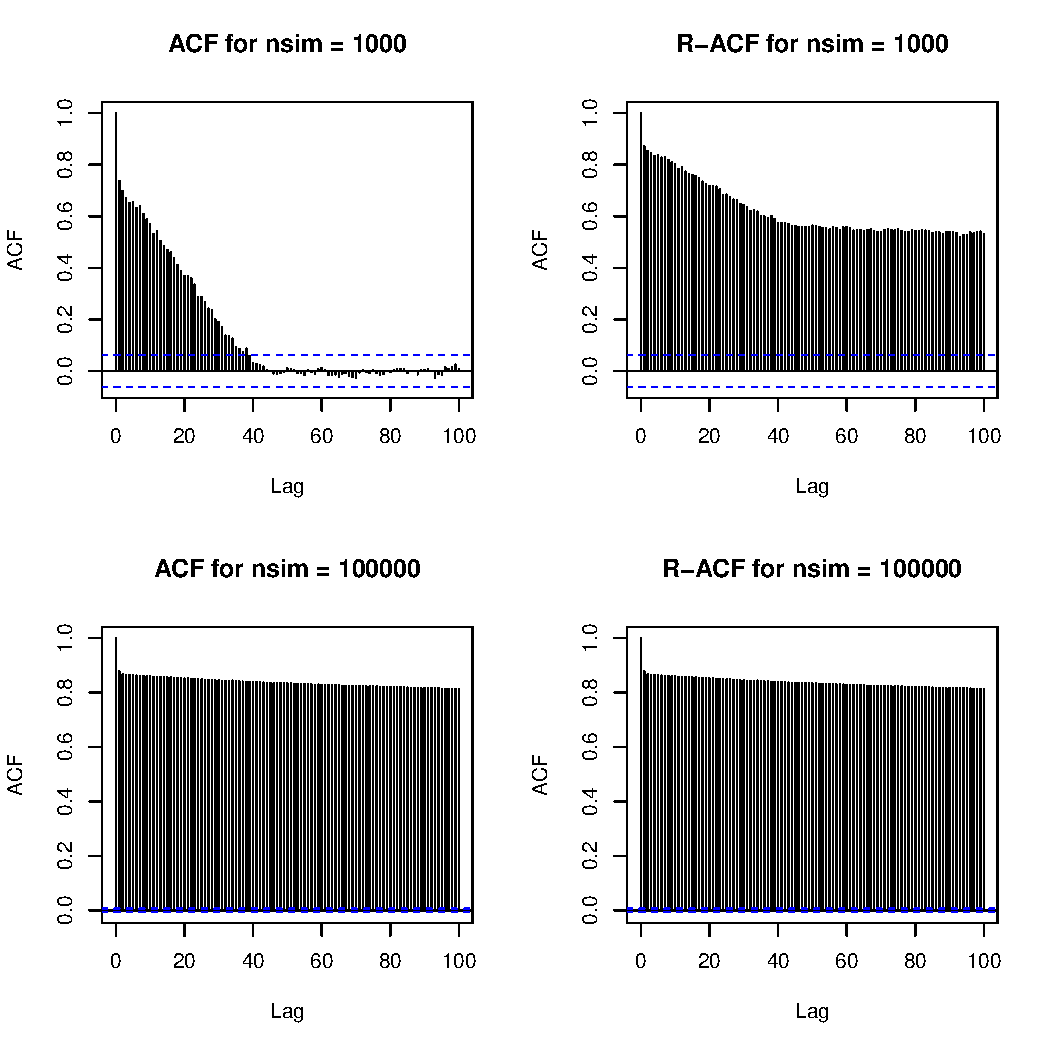
\includegraphics[width = 0.55\textwidth]{plots/spatio-acf.pdf}
    \caption{ACF and G-ACF for the first component of the first chain.}
    \label{fig:spatio-acf_G-fl}
\end{figure}
We run two parallel Markov chains from randomly chosen starting points and present the resulting ACF and G-ACF in Figure \ref{fig:spatio-acf_G-fl}. The early G-ACF estimates are far closer to the G-ACF and ACF estimates at $10^5$.

 % it is evident that the chains have not explored the sample space well. Hence for $10^3$ samples ACF severely underestimates the autocorrelations whereas G-ACF gives more realistic estimates. For a large sample size of $10^5$, the Markov chains have mixed properly and therefore, both the estimators are approximately alike.

\subsection{Network crawling}

% \cite{handcock2008statnet} implemented an exponential-family random graph modelling (ERGM) on network data in the package . 

The \texttt{faux.magnolia.high} dataset available in the \texttt{ergm} \texttt{R} package represents a simulated within school friendship network based on Ad-Health data (\cite{resnick1997protecting}). The school communities represented by the network data are located in the southern United States. Each node represents a student and each edge represents a friendship between the nodes it connects. 

The goal is to draw each node uniformly from the network by using a network crawler. \cite{nilakanta2019ensuring} modified the data by removing 1,022 out of 1,461 nodes to obtain a well-connected graph. This resulting social network has 439 nodes and 573 edges. We use a Metropolis-Hastings algorithm with a simple random-walk  proposal suggested by \cite{gjoka2011practical}. The stationary distribution for this algorithm is a uniform distribution over the nodes. 
% , i.e. $\lambda(i) = 1/n$ for all $i \in V$.  The Metropolis-Hastings transition kernel for this method is

% Let $V$ denote the non-empty set of countable nodes, $E \subseteq V \times V$ denote the set of edges, and $G = (V,E)$ denote the network. We are interested in exploring all the nodes uniformly, i.e. sample from a uniform distribution over $V$. Let $\lambda$ denote a uniform distribution over $V$  let $h: V \to \mathbb{R}^p$ map each node to certain features of interest. If $X \sim \lambda$, we wish to calculate the expected value of $h(X)$ with respect to $\lambda$ given by

% \[
% \mathbb{E}[h(X)]_{\lambda} = \dfrac{1}{n}\sum_{x \in V}h(x).
% \]

% Here n is the set cardinality of $V$. 



% \[
% P(i,j) = \begin{cases}
%              \dfrac{1}{d_i} \min\left\{1, d_i{d_j}^{-1}\right\} & \textrm{if $j$ is a neighbor of $i$}  \\
%              1 - \sum_{k \neq i} d_i^{-1} \min \left\{1, {d_i}{d_k}^{-1}\right\} & \textrm{if } j = i\\
%              0 & \textrm{otherwise}.
%         \end{cases}
% \]

% Table (blah) shows the population parameters we are interested in estimating using MCMC methods.  The G-e and sex parameters are estimated as proportion of whites and females in the sample respectively. 

We start two parallel Markov chains from two students belonging to different {\color{red}G-es ???} and study its impacts on the average features of their immediate social group. 
% It is hypothesized that students from certain communities tend to engage more with students of same or other marginally represented communities. We believe that this "selective networking" might cause formation of clusters in the network wherein students within a cluster engage more with each other than with the students outside it. Given that the graph is well-connected, the Markov chains will eventually explore all the nodes. 


\singlespacing
\bibliographystyle{apalike}
\bibliography{sample}
\end{document}
